\documentclass[11pt]{article}
\usepackage{deauthor}
\usepackage{enumitem}
\usepackage{algorithmic}
\usepackage{algorithm}
\usepackage{xcolor}
\usepackage{xspace}
\usepackage{graphicx}
%\usepackage[caption=false]{subfig}
\usepackage{footnote}
\usepackage{hyperref}
\usepackage{multirow}
\usepackage{subfig}
\usepackage{enumitem}
\usepackage{comment}

\usepackage{dsfont}
\usepackage{wrapfig}
\usepackage{amssymb}

\usepackage{booktabs} % For formal tables

%\usepackage{etoolbox}
%\apptocmd{\thebibliography}{\scriptsize}{}{}

%\usepackage{etoolbox}
%\apptocmd{\thebibliography}{\scriptsize}{}{}
\usepackage{multirow}
%\usepackage{graphicx}
\usepackage{balance}  % for  \balance command ON LAST PAGE  (only there!)

\usepackage{color}
\usepackage{xcolor}
\usepackage{amssymb}% http://ctan.org/pkg/amssymb
\usepackage{pifont}% http://ctan.org/pkg/pifont

\usepackage{pifont}
\usepackage{url}

\usepackage{booktabs} % For formal tables

\usepackage{enumitem}
\usepackage{amsmath}
%\usepackage[linesnumbered,ruled]{algorithm2e}
% \usepackage[linesnumbered,ruled,vlined]{algorithm2e}


\usepackage{graphicx}
% \usepackage[font=scriptsize]{subfig}
% \usepackage[font=small,labelfont=bf]{caption}
%\usepackage{subfigure}
\usepackage{epsfig}

% For statistical figure
\usepackage{tikz}
\usetikzlibrary{snakes}

% \theoremstyle{definition}
% \newtheorem{definition}{Definition}
\newcommand{\Hammer}{\emph{iQAN}\xspace}
\newcommand{\SeqFullName}{Best-First Search\xspace}
\newcommand{\SeqShortName}{\emph{BFiS}\xspace}
\newcommand{\KNNS}{$K$-NNS\xspace}
\newcommand{\DeltaStep}{\emph{$\Delta$-Step}\xspace}
\newcommand{\PunchStarter}[1]{\noindent\textbf{#1}\xspace}

\definecolor{SeafoamGreen}{RGB}{159, 226, 191}
\definecolor{Peach}{RGB}{255, 203, 164}

\newcommand{\algoname}{HM-ANN\xspace}
\newcommand{\name}{HM-ANN\xspace}

\begin{document}


\title{Querying Time-Series Data: A Comprehensive Comparison of Distance Measures}

\author{John Paparrizos$^*$, Chunwei Liu$\ddagger$, Aaron J. Elmore$\dagger$, Michael J. Franklin$\dagger$\\
  $^*$The Ohio State University, paparrizos.1@osu.edu \\
  $\dagger$University of Chicago \\
  $\ddagger$Massachusetts Institute of Technology\\
}


\maketitle
\renewcommand\thesection{\arabic{section}}
\setcounter{section}{0}
\setcounter{figure}{0}
\setcounter{table}{0}

\begin{abstract}
%In a multitude of scientific and industrial applications, the basis for most data analyses involves the querying of time-series. 
Distance measures are core building blocks in time-series analysis and the subject of active research for decades. Unfortunately, the most detailed experimental study in this area is outdated (over a decade old) and, naturally, does not reflect recent progress. Importantly, this study (i) omitted multiple distance measures, including a classic measure in the time-series literature; (ii) considered only a single time-series normalization method; and (iii) reported only raw classification error rates without statistically validating the findings, resulting in or fueling four misconceptions in the time-series literature. Motivated by the aforementioned drawbacks and our curiosity to shed some light on these misconceptions, we comprehensively evaluate \textcolor{black}{$71$} time-series distance measures. Specifically, our study includes (i) $8$ normalization methods; (ii) $52$ lock-step measures; (iii) $4$ sliding measures; (iv) $7$ elastic measures; \textcolor{black}{(v) $4$ kernel functions; and (vi) $4$ embedding measures}. We extensively evaluate these measures across $128$ time-series datasets using rigorous statistical analysis. For the most promising measures, we present an accuracy-to-runtime analysis and summarize recent progress on a generalized lower bounding measure that accelerates all elastic distances. Our findings debunk four long-standing misconceptions that significantly alter the landscape of what is known about existing distance measures. With the new foundations in place, we discuss open challenges and promising directions.
\end{abstract}


\section{Introduction}
\label{john_sec:intro}

%Problem
The understanding of a multitude of natural or human-made processes involves the analysis of high-dimensional observations over time.  The recording of such time-varying measurements leads in an ordered sequence of data points called {\em time series} \cite{palpanas2015data,paparrizos2018fast}. In the last decades, time-series analysis has become increasingly prevalent, affecting virtually all scientific disciplines and their corresponding industries \cite{UCRArchive2018,liu2023amir,krishnan2019artificial,paparrizos2016detecting,paparrizos2016screening,mckeown2016predicting,goel2016social}. With sensors and devices becoming increasingly networked and with the explosion of Internet-of-Things (IoT) applications, the volume of produced time series is expected to continue to rise \cite{mahdavinejad2017machine,paparrizos2021vergedb,jiang2020pids,jiang2021good,liu2021decomposed}. This growth and ubiquity of time series generates tremendous interest in the extraction of meaningful knowledge from time series \cite{dziedzic2019band,paparrizos2019grail}.


% Interesting and Important
The basis for most analytics over time series involves the detection of similarities between time series. The measurement of similarity, through a {\em distance or similarity measure}, is the most fundamental building block in time-series data mining, fueling tasks such as querying \cite{agrawal1993,ding2008querying,paparrizos2023accelerating,paparrizos2022fast}, indexing \cite{echihabi2018lernaean,Keogh2001locally,zoumpatianos2016ads}, clustering \cite{paparrizos2023odyssey,keogh2005clustering,paparrizos2015k,paparrizos2017fast,bariya2021k}, classification \cite{bagnall2017great,paparrizos2019grail,ratanamahatana2004making,ye2009time}, motif discovery \cite{mueen2009exact,linardi2018scalable,yeh2016matrix}, and anomaly detection \cite{dallachiesa2014top,paparrizos2022tsb,paparrizos2022volume,boniol2021sand,boniol2022theseus,boniol2021sandaction,boniol2023edbt,sylligardos2023choose}. In contrast to other data types where distance measures often process observations independently, for time series, distance measures consider sequences of observations together. This characteristic complicates the definition of distance measures for time series and, therefore, it is desirable to study the factors that determine their effectiveness.

% Why it's hard
The difficulty in formalizing accurate distance measures stems from the inability to express precisely the notion of similarity. As humans we easily recognize perceptually similar time series, by ignoring a variety of distortions, such as fluctuations, misalignments, and stretching of observations. However, it is challenging to derive definitions to reflect the similarity for mathematically non-identical time series \cite{esling2012time}. Due to that difficulty and the need to handle the variety of distortions, dozens of distance measures have been proposed \cite{assfalg2006similarity,berndt1994using,chen2004marriage,chen2005robust,chen2007spade,ding2008querying,Faloutsos1994fast,frentzos2007index,morse2007efficient,stefan2013move,vlachos2002discovering,paparrizos2015k,paparrizos2019grail,sakoe1978dynamic}.

% Why it hasn't been solved / what's wrong
Despite this abundance of time-series distance measures and their implications in the effectiveness for a multitude of time-series tasks, less attention has been given in their comprehensive experimental validation. Specifically, in the past two decades, only a single comprehensive experimental evaluation has been dedicated to studying the accuracy of 9 influential time-series distance measures over 38 datasets \cite{ding2008querying}. Unfortunately, this study suffers from three main drawbacks: (i) this study omitted multiple distance measures, including one of the most classic measures in the time-series literature, namely, the cross-correlation measure \cite{papoulis1962fourier,bracewell1965pentagram}; (ii) this study considered only a single time-series normalization method; and (iii) this study reported raw classification error rates without performing any rigorous statistical analysis to assess the significance of the findings. Therefore, the analysis is incomplete, and, the findings might not be conclusive. Importantly, this study is now outdated (more than a decade old), and, naturally, it does not reflect recent progress. Considering the previous drawbacks as well as the remarkable interest in time-series analysis, we believe it is critical to revisit this subject.

However, our effort is not only motivated by the necessity to address the aforementioned issues or to extend the previous study with newer datasets and distance measures. Instead, the thorough experimental evaluation of time-series distance measures that we present in this paper is the byproduct of our attempt to challenge four long-standing misconceptions (see $\mathcal{M}1-\mathcal{M}4$ in Section \ref{john_sec:perceptions}) that have appeared in the time-series literature. These misconceptions are concerned with the (i) normalization of time series; (ii) identification of the state-of-the-art distance measure in every category of measures; \textcolor{black}{(iii) performance of the omitted measures against state-of-the-art measures;} and (iv) detection of the most powerful category of measures. Such misconceptions originated from several influential papers \cite{agrawal1993,Faloutsos1994fast,goldin1995similarity,berndt1994using,shieh2008sax}, some of which date back a quarter of a century, and are fueled by recent inconclusive findings \cite{ding2008querying} as well as successive claims in the literature that we discuss later. Considering how widely cited and impactful these papers are, we believe it is risky not to challenge such persistent misconceptions that might disorientate newcomer researchers and practitioners. 

Motivated by the aforementioned issues and our curiosity to shed some light on these misconceptions, we conduct a comprehensive experimental evaluation to validate the effectiveness of \textcolor{black}{ $71$ time-series distance measures. These distance measures belong to five categories: (i) $52$ {\em lock-step} measures, which compare the $i$th point of one time series with the $i$th point of another; (ii) $4$ {\em sliding} measures, which are the sliding versions of lock-step measures when comparing one time series with all shifted versions of the other; (iii) $7$ {\em elastic} measures, which create a non-linear mapping between time series by comparing one-to-many points in order to align or stretch points; (iv) $4$ {\em kernel} measures, which use a function (with lock-step, sliding, or elastic properties) to implicitly map data into a high-dimensional space; and (v) $4$ {\em embedding} measures, which exploit distance or kernel measures indirectly for constructing new representations for time series.} In addition, we consider $8$ normalization methods for time series. %Table \ref{john_tab:studystats}, summarizes our comprehensive evaluation and compares some statistics against the decade-old influential study \cite{ding2008querying}.

We perform an extensive evaluation of these distance measures across $128$ datasets \cite{UCRArchive2018} and compare their classification accuracy obtained from one-nearest-neighbor classifiers ($1$-NN) under both supervised and unsupervised settings. We conduct a rigorous statistical validation of our findings by employing two statistical tests to assess the significance of the differences in classification accuracy when comparing pairs of measures or multiple measures together. In summary, our study identifies (i) normalization methods leading to significant improvements in a number of distance measures; (ii) new lock-step measures that significantly outperform the current state of the art; (iii) an omitted baseline that most highly popular elastic measures do not outperform; and (iv) \textcolor{black}{new elastic and new kernel measures} that significantly outperform the current state of the art. These findings debunk the four long-standing misconceptions and alter the landscape of what is known about existing measures. 

%We take several steps to ensure the reproducibility of our findings and we provide the raw results in an interactive website to ease exploration \cite{TSDistEval2019}. , including using publicly available datasets, making our source code available, and by providing the raw results in an interactive website to ease exploration



We start with the description of the four misconceptions in the literature (Section \ref{john_sec:perceptions}) and we review the relevant background (Section \ref{john_sec:preliminaries}). Then, we present our contributions: 
\begin{itemize}[noitemsep,topsep=0pt,parsep=0pt,partopsep=0pt,leftmargin=0.5cm]
	\item We explore for the first time $8$ normalization methods along $56$ distance measures (Section
	\ref{john_sec:normalizations}).
	\item We study $52$ lock-step distance measures (Section
	\ref{john_sec:lockstep}).
	\item We investigate $4$ classic sliding measures omitted from every previous evaluation (Section \ref{john_sec:sliding}).
	\item We compare $7$ elastic measures under supervised and unsupervised settings (Section \ref{john_sec:elastic}).
	\item We study for the first time $4$ kernel (Section \ref{john_sec:kernel}) and $4$ embedding distance measures (Section \ref{john_sec:embedded}).
	\item We present an accuracy-to-runtime analysis (Section \ref{john_sec:overall}).
 	\item We summarize recent progress towards accelerating the strongest elastic distances via the use of lower bounding measures (Section \ref{john_sec:accelerating}).
\end{itemize}
\noindent Finally, we discuss new directions (Section \ref{john_sec:futurework}) and conclude with the implications of our work (Section \ref{john_sec:conclusions}). An earlier version of the paper has been published in ACM SIGMOD 2020 \cite{paparrizos2020debunking}.

\section{The Four Misconceptions}
\label{john_sec:perceptions}

In this section, we describe four misconceptions that have appeared in the time-series literature. 

These misconceptions have originated in part from several influential papers \cite{agrawal1993,Faloutsos1994fast,goldin1995similarity,berndt1994using,shieh2008sax}. Subsequently, these misconceptions were fueled by a comprehensive study of time-series distance measures \cite{ding2008querying} as well as dozens of subsequent papers in the literature trusting its findings. Even though an extension of this study appeared five years later \cite{wang2013experimental}, this newer version focused on elaborating on the previous results. %This updated version did not include any omitted or newer distance measures neither conducted the missing statistical analysis. 
Recent studies that have focused on time-series classification \cite{bagnall2017great,lines2015time} performed a statistical analysis of several classifiers, including the distance measures in \cite{ding2008querying,wang2013experimental}. Unfortunately, these studies only considered supervised tuning of necessary parameters, which does not reflect the use of distance measures for similarity search \cite{echihabi2018lernaean}. Importantly, some results in \cite{bagnall2017great} contradict other results in \cite{lines2015time}, which, in turn, validated claims that there is no significant difference between the evaluated elastic measures \cite{ding2008querying,wang2013experimental}. Interestingly, the improved accuracy found for some measures was attributed to the evaluation framework used while otherwise it was claimed to be undetectable \cite{bagnall2017great}. Considering such apparent difficulties in providing conclusive evidence for this important subject, it is not surprising that the following misconceptions have persisted for so long. 

Before we dive into the details, we emphasize that we do not believe or imply that any of these misconceptions were created on purpose. On the contrary, we believe that they are based on evidence, trends, and resources available at the given point in time. We describe the four misconceptions in the form of answers to questions a newcomer researcher would likely identify by studying the literature.
\newline \textbf{$\mathcal{M}1$: How to normalize time series?} The consensus is to use the $z$-score or $z$-normalization method. Starting with the work of Goldin and Kanellakis \cite{goldin1995similarity}, a follow-up of the two seminal papers for sequence \cite{agrawal1993} and subsequence \cite{Faloutsos1994fast} search in time-series databases, that suggested first to normalize the time series to address issues with scaling and translation, $z$-normalization became the prevalent method to preprocess time series. Despite the proposal of alternative methods the same year \cite{lin1995fast}, the $z$-normalization was subsequently preferred as the suggested transformations are also applicable to the widely popular Fourier representation \cite{agrawal1993,Faloutsos1994fast,rafiei1997similarity}. Due to the ubiquity of $z$-normalization, a valuable resource for time series, the UCR Archive \cite{UCRArchive2018}, offered until recently the datasets in their $z$-normalized form. To the best of our knowledge, no study has ever extensively evaluated normalization methods for time series. We review $8$ approaches in Section \ref{john_sec:normalizations} and study their performance in Sections \ref{john_sec:lockstep} and \ref{john_sec:sliding}.
\newline \textbf{$\mathcal{M}2$: Which lock-step measure to use?} The consensus is to use the Euclidean distance (ED). ED was the method of choice in the first paper for sequence search in time series \cite{agrawal1993} due to its usefulness in many cases and its applicability over feature vectors. Considering that ED is straightforward to implement, parameter-free, efficient, as well as tightly connected with the Fourier representation and widely supported by indexing mechanisms (in contrast to other $L_p$-norm variants \cite{yi2000fast}), there is no surprise about its popularity. Besides, evidence that with increased dataset sizes, the classification error of ED converges to the error of more accurate measures \cite{shieh2008sax}, justified its use from virtually all current time-series indexing methods \cite{echihabi2018lernaean}. (Our results in Section \ref{john_sec:overall} suggest that classification error of ED may not always converge to the error of more accurate measures, at least not always with the same speed of convergence.) In Section \ref{john_sec:lockstep}, we evaluate $52$ lock-step measures.
\newline \textbf{$\mathcal{M}3$: Are elastic better than sliding measures?} The answer is currently unknown. Despite the wide popularity of the cross-correlation measure, also known as sliding Euclidean or dot product distance, in the signal and image processing literature \cite{brown1992survey}, cross-correlation has largely been omitted from distance measure evaluations. We believe two factors are responsible for that. First, cross-correlation was considered in the seminal paper \cite{agrawal1993} as a typical similarity measure, but ED was preferred instead because (i) cross-correlation reduces to ED; and (ii) for the aforementioned reasons in $\mathcal{M}2$. Second, in the introduction of Dynamic Time Warping (DTW) \cite{berndt1994using}, an elastic measure, as an alternative to ED a year later, no comparison was performed against cross-correlation, an obvious baseline. Subsequently, virtually all research on that subject focused either on lock-step or elastic measures \cite{esling2012time,echihabi2018lernaean}, with a few exceptions \cite{li1996hierarchyscan,sakurai2005braid,paparrizos2015k}. Interestingly, cross-correlation was not considered as a baseline method in any of the proposed elastic measures \cite{chen2004marriage,chen2005robust,chen2007spade,morse2007efficient,stefan2013move,vlachos2002discovering}, neither in any of the experimental evaluations of distance measures discussed previously \cite{ding2008querying,wang2013experimental,lines2015time,bagnall2017great}. Strangely, cross-correlation was also omitted from many popular surveys \cite{esling2012time,ralanamahatana2005mining}. Therefore, it remains unknown if elastic measures outperform sliding measures. We study $4$ sliding measures in Section \ref{john_sec:sliding} and analyse their performance against elastic measures in Section \ref{john_sec:elastic}.
\newline \textbf{$\mathcal{M}4$: Is {\em DTW} the best elastic measure?} The general consensus that has emerged is yes. Since the introduction of DTW as a distance measure for time series \cite{berndt1994using}, DTW has inspired the exploration of edit-based distances and it is widely used as the baseline method for this problem \cite{chen2004marriage,chen2005robust,chen2007spade,morse2007efficient,stefan2013move,vlachos2002discovering,lines2015time,paparrizos2015k,bagnall2017great}. It is not uncommon to identify statements even in the abstracts of papers that $1$-NN with DTW is exceptionally difficult to outperform \cite{xi2006fast,petitjean2011global,petitjean2014dynamic,petitjean2016faster}. Such statements have been backed over the years by the aforementioned extensive evaluations, which conclude that (i) the accuracy of other elastic measures is very close to that of DTW \cite{ding2008querying,wang2013experimental}; (ii) there is no significant difference in the accuracy of elastic measures \cite{lines2015time}; and (iii) that it is ``a little embarrassing'' that most classifiers do not outperform $1$-NN with DTW \cite{bagnall2017great}. Therefore, there is little space to doubt that DTW is the best elastic measure. To study that misconception, we validate $7$ elastic measures in Section \ref{john_sec:elastic}.

\textcolor{black}{To complete the analysis and capture recent progress, we also include kernel measures and embedding measures in our evaluation (Sections \ref{john_sec:kernel} and \ref{john_sec:embedded})}. With the detailed presentation of the four misconceptions, we believe we have now convinced the reader that these misconceptions are not based on any personal biases but, instead, have originated naturally along with the evolution of this area. However, it is risky to not challenge their validity, which may result in confusion for newcomer researchers and practitioners and discourage them from tackling problems in that area. Importantly, it is surprising to consider that half a century of scientific progress has not resulted in any significant improvements over ED or the 50-year-old DTW \cite{sakoe1971dynamic}.

Next, we review the relevant background required to validate the accuracy of the normalization methods and distance measures. Even though the efficiency of measures is another important factor of their effectiveness, there are many ways to accelerate each measure, ranging from hardware-aware implementations to algorithmic solutions such as the use of indexing or comparison pruning. We refer the reader to an excellent recent study of data-series similarity search \cite{echihabi2018lernaean}, which shows the level of detail required to only evaluate ED. \textcolor{black}{Therefore, we leave such detailed study for future work but we present an accuracy-to-runtime analysis in Section \ref{john_sec:overall}.}

\vspace*{-0.1cm}
\section{Preliminaries and background}
\label{john_sec:preliminaries}

In this section, we review the necessary background for our experimental evaluation.
\newline \textbf{Terminology and definitions: } We consider a time-series dataset as a set of $n$ real-valued vectors $X=[\vec{x}_1,\ldots,\vec{x}_n]^\top\!\in\!\mathbb{R}^{n \times m}$, where each time series, $\vec{x}_i\!\in\!\mathbb{R}^{m}$, is an $m$-dimensional ordered sequence of data points. From this definition, it becomes clear that we consider {\em univariate} time series of equal length, where each of these points is a scalar. Following the previous evaluations \cite{ding2008querying,wang2013experimental,bagnall2017great}, we consider that the sampling rates of all time series are the same and omit the discrete time stamps. 
%Finally, the time series in each dataset have equal length, but among datasets, the length varies.
\newline \textcolor{black}{\textbf{Datasets: } To conduct our extensive evaluation, we use one of the most valuable public resources in the time-series data mining literature, the UCR Time-Series Archive \cite{UCRArchive2018}. This archive contains the largest collection of class-labeled time-series datasets. Currently, the archive consists of $128$ datasets and includes time series from sensor readings, image outlines, motion capture, spectrographs, medical signals, electric devices, as well as simulated time series. Each dataset contains from $40$ to $24,000$ time series, the lengths vary from $15$ to $2,844$, and each time series is annotated with a single label. The majority of the datasets are already $z$-normalized and we apply the same normalization to all datasets.}

The latest version of the archive has deliberately left a small number of datasets containing time series with varying lengths and missing values to reflect the real world. Following the recommendation of the authors of the archive, who performed similar steps to report classification accuracy numbers on the UCR archive website \cite{UCRArchive2018}, we resample shorter time series to reach the longest time series in each dataset and we fill missing values using linear interpolation. Through these steps, we make the new datasets compatible with previous versions of the archive \cite{UCR2018Fixes}.
\newline \textbf{Evaluation framework: } Following the previous studies \cite{ding2008querying,bagnall2017great}, we also employ the $1$-NN classifier in our evaluation framework, with important differences. $1$-NN classifiers are suitable methods for distance measure evaluation for several reasons \cite{ding2008querying}. Specifically, $1$-NN classifiers: (i) resemble the problem solved in time-series similarity search \cite{echihabi2018lernaean}; (ii) are parameter-free and easy to implement; (iii) dependent on the choice of distance measure; and (iv) provide an easy-to-interpret (classification) accuracy measure, which captures if the query and the nearest neighbor belong to the same class. 

A critical step for the effectiveness of classifiers is the splitting of a dataset into training and test sets. Previous studies \cite{ding2008querying,wang2013experimental,bagnall2017great} used the $k$-cross-validation resampling procedure, which produces $k$ groups of time series, tunes necessary parameters on the $k-1$ groups, and evaluates the distance measures using the group of time series left. Strangely, \cite{ding2008querying,wang2013experimental} tuned parameters only on a single group and evaluated the distance measures using the $k-1$ groups, which contradicts the common practice. In \cite{bagnall2017great}, the improved accuracy of some measures is attributed to such a resampling procedure, while otherwise, it was claimed to be undetectable. Therefore, to eliminate biases from resampling, we respect the split of training and test sets provided by the UCR archive as well as the class distribution in the datasets (i.e., some datasets contain the same number of time series in each class while other datasets contain imbalanced classes). This decision makes our evaluation framework deterministic and enables reproducibility. Refer to \cite{paparrizos2020debunking}  for further details on our evaluation settings.

%More formally, given a matrix $F=[\vec{f}_1,\ldots,\vec{f}_p]^\top\!\in\!\mathbb{R}^{p \times m}$ with the $p$ time series in the training set, a matrix $G=[\vec{g}_1,\ldots,\vec{g}_r]^\top\!\in\!\mathbb{R}^{r \times m}$ with the $r$ time series in the test set, and any choice of distance measure, $d(\cdot,\!\cdot)$, our $1$-NN classifier relies on two dissimilarity matrixes to produce the final classification accuracy. Specifically, matrix $W\!\in\!\mathbb{R}^{p\times p}$ contains the dissimilarity values between all pairs of time series in the training set, with $W_{ij}=d(\vec{f}_i,\vec{f}_j)\,\forall\,\vec{f}_i,\vec{f}_j\!\in\!F$, whereas matrix $E\!\in\!\mathbb{R}^{r\times p}$ contains the dissimilarity values between each time series in the test set with each time series in the training set, with $E_{ij}=d(\vec{g}_i,\vec{f}_j)\,\forall\,\vec{g}_i\!\in\!G,\,\vec{f}_j\!\in\!F$. 
%Algorithm \ref{john_alg:1nn} shows the pseudocode of our $1$-NN classifier that evaluates the {\em test} accuracy given a matrix $E$ (as well as vectors $FL$ and $GL$ containing the class labels of $F$ and $G$, respectively). By providing as input, a matrix $W$ (as well as two times the vector $FL$ containing the class labels of $F$), the same algorithm computes the leave-one-out {\em training} accuracy, which enables parameter tuning. With this setup, we decouple the processes of distance matrix computation, parameter tuning, and distance measure evaluation. Importantly, it facilitates easy distribution of the computation of the dissimilarity matrixes for different parameters and avoids the need to find the appropriate $k$ value to perform $k$-cross-validation, which is another factor that might have affected the findings in the previous studies \cite{ding2008querying,bagnall2017great}.

\noindent \textbf{Statistical analysis: } To assess the significance of the differences in accuracy, we employ two statistical tests to validate the pairwise comparisons of measures and the comparisons of multiple measures together. Specifically, following the highly influential \cite{demvsar2006statistical}, we use the Wilcoxon test \cite{wilcoxon1945individual} with a 95\% confidence level to evaluate pairs of measures over multiple datasets, which is more appropriate than the t-test \cite{rice2006mathematical}. As with pairwise tests we cannot reason about multiple measures together and following \cite{demvsar2006statistical}, we also use the Friedman test \cite{friedman1937use} followed by the post-hoc Nemenyi test \cite{nemenyi1963distribution} to compare multiple measures over multiple datasets and report statistical significant results with 90\% confidence level (because these tests require more evidence than Wilcoxon). 
\newline \textcolor{black}{ \textbf{Availability of code and results: } We implemented the evaluation framework in Matlab, with imported C and Java codes for several distance measures. To ensure the reproducibility of our findings, we make the code available.\footnote{\url{https://github.com/TheDatumOrg/TSDistEval}}}
\newline \textcolor{black}{ \textbf{Environment: } We ran our experiments on 15 identical servers: Dual Intel(R) Xeon(R) Silver 4116 CPU @ 2.10GHz and 196GB RAM. Each server has 24 physical cores (12 per CPU), which provided us with 360 cores for four months}. 

Next, we start with the study of normalization methods.

\begin{figure*}[t!]
	\vspace*{-0.3cm}
	\centering
	\subfloat[$z$-score]{{\label{john_fig:norm1}}{\includegraphics[height=3cm,width=4.2cm]{submissions/John2023/figures/Normzscore-crop.pdf}
	}}%
	%\qquad
	\subfloat[MinMax]{{\label{john_fig:norm2}}{\includegraphics[height=3cm,width=4.2cm]{submissions/John2023/figures/Normminmax-crop.pdf}
	}} 
		\subfloat[UnitLength]{{\label{john_fig:norm3}}{\includegraphics[height=3cm,width=4.2cm]{submissions/John2023/figures/Normunitlength-crop.pdf}
	}} 
		\subfloat[MeanNorm]{{\label{john_fig:norm4}}{\includegraphics[height=3cm,width=4.2cm]{submissions/John2023/figures/Normmeannorm-crop.pdf}
	}} \vspace*{-0.3cm}
	\qquad
		\subfloat[MedianNorm]{{\label{john_fig:norm5}}{\includegraphics[height=3cm,width=4.2cm]{submissions/John2023/figures/Normmediannorm-crop.pdf}
	}} 
		\subfloat[AdaptiveScaling]{{\label{john_fig:norm6}}{\includegraphics[height=3cm,width=4.2cm]{submissions/John2023/figures/Normadaptive-crop.pdf}
	}} 
		\subfloat[Logistic]{{\label{john_fig:norm7}}{\includegraphics[height=3cm,width=4.2cm]{submissions/John2023/figures/Normsigmoid-crop.pdf}
	}} 
		\subfloat[Tanh]{{\label{john_fig:norm8}}{\includegraphics[height=3cm,width=4.2cm]{submissions/John2023/figures/Normtanh-crop.pdf}
	}} 
	\vspace*{-0.2cm}
	\caption{Example of how each of the $8$ normalization methods transforms time series of ECGFiveDays \cite{UCRArchive2018}.}%
    %\vspace*{-0.2cm}
	\label{john_fig:normalizations}%
\end{figure*}

%\vspace*{-0.1cm}
\section{Time-Series Normalizations}
\label{john_sec:normalizations}
In this section, we review $8$ normalization methods. As we discussed earlier, a critical issue when comparing time series is how to handle a number of distortions that are characteristic of the time series. For complex distortions, sophisticated distance measures are required as offering invariances to such distortions is not trivial, which explains the proliferation of distance measures in the literature. However, in several cases, a simple preprocessing step is generally sufficient, as we see next.

Consider the following two examples \cite{goldin1995similarity}: (i) two products with similar sales patterns but different sales volume; and (ii) temperatures of two days starting at different values but exhibiting the exact same pattern. The first is an example of the difference in {\em scale} between two time series, whereas the second is an example of the difference in {\em translation}. Despite such differences, in many cases, it is useful to recognize the similarity between time series. Formally, for any constants $a$ (scale) and $b$ (translation), linear transformations in time series of the form $a\vec{x}+b$ should not affect their similarity. 

Several methods have been proposed to handle these popular distortions. {\em Normalization} methods transform the data to become normally distributed, whereas {\em standardization} methods place different data ranges on a common scale. In the machine-learning literature, feature {\em scaling} is also used to refer to such methods. In practice, all terms are used interchangeably to refer to some data transformation. 

We consider $8$ popular normalization methods in our study, namely, $z$-score, min-max (MinMax), Mean (MeanNorm), Median (MedianNorm), Unit length (UnitLength), Adaptive scaling (AdaptiveScaling), Logistic or Sigmoid (Logistic), and Hyperbolic tangent (Tanh) normalization. (Please refer to \cite{paparrizos2020debunking} for more details and their mathematical formulas.) Figure \ref{john_fig:normalizations}, shows an example of how each one of the previously described normalization methods transforms a pair of time series from ECGFiveDays \cite{UCRArchive2018}. We observe that in some cases, the differences are only visible in the range of values (e.g., $z$-score vs. UnitLength), but, in others, the visual effect is more distinct (e.g., MinMax, MeanNorm, and AdaptiveScaling). The most unexpected visual effects come from the two non-linear transformations (i.e., Logistic and Tanh). Next, we evaluate $8$ methods along with the $52$ lock-step measures.

\section{Time-Series Lock-Step Distances}
\label{john_sec:lockstep}

In this section, we study $52$ lock-step measures that have been proposed across different disciplines.

Distance measures provide a numerical value to quantify how distant are pairs of objects represented as points, vectors, or matrixes. Due to the difficulty in formalizing the notion of similarity, as well as the need to handle a variety of distortions and applications, hundreds of distance measures have been proposed in the literature. This proliferation of distance measures across different scientific areas has resulted in multi-year efforts to organize this knowledge into dictionaries \cite{deza2006dictionary} and encyclopedias \cite{deza2009encyclopedia}. 

As it is understandable, not all of these measures are applicable to time-series data. Thankfully, different endeavors have already been conducted to identify appropriate measures for a variety of tasks across different fields \cite{zezula2006similarity,gavin2003statistical}. An influential study \cite{cha2007comprehensive} identified $50$ lock-step distance measures that we adapt in our evaluation of time-series distance measures. We note that a previous study \cite{giusti2013empirical} evaluated a subset of these measures ($45$) using $1$-NN over $42$ datasets from the UCR archive and concluded that there is no significant differences between these lock-step distance measures.

Unfortunately, we identified issues with this study. First, several of the evaluated measures are known to be equivalent to each other and, therefore, they should provide identical classification accuracy results. For example, this is the case for the Euclidean distance and the inner product (or Pearson's correlation), which under $z$-normalization, they should provide the same accuracy numbers. Second, several distance measures were not properly implemented, resulting in using as distance values either the real part of complex numbers or the first value of a normalized vector of the input time series. Therefore, the analysis of these lock-step measures is incomplete, and the findings are inconclusive.

In our study, we have carefully re-implemented all $50$ distance measures from \cite{cha2007comprehensive}. The distance measures belong to $7$ different families of measures: (1) $4$ measures belong to the $L_p$ Minkowski family; (2) $6$ measures belong to the $L_1$ family; (3) $7$ measures belong to the {\em Intersection} family; (4) $6$ measures belong to the {\em Inner Product} family; (5) $5$ measures belong to the {\em Fidelity} family; (6) $8$ measures belong to the $L_2$ family; and (7) $6$ measures belong to the {\em Entropy} family. Apart from these $42$ measures, we also consider the $3$ measures that utilize ideas from multiple other measures ({\em Combinations}) as well as $5$ measures proposed in the survey but not reported in the literature (until that point).

Besides these measures, we also include two measures that have substantial differences from the previous lock-step measures. Specifically, DISSIM \cite{frentzos2007index} defines the distance as a definite integral of the function of time of the ED in order to take into consideration different sampling rates of time series. This computationally expensive operation can be approximated by a modified version of ED that considers in the distance of the $i$th points the $i+1$th points, which is a form of a smoothing operation. Finally, the adaptive scaling distance (ASD), embeds internally the AdaptiveScaling normalization with an inner product measure to compare time series under optimal scaling \cite{chu1999fast,yang2011patterns}. 
\newline \textbf{Evaluation of lock-step measures: } For all mathematical formulas, we refer the reader to the previous survey \cite{cha2007comprehensive}. We evaluate $52$ distance measures and their combinations with $8$ normalization methods using our $1$-NN classifier over $128$ datasets (see Section \ref{john_sec:preliminaries}). From all combinations of distance measures and normalization methods ($52\cdot8=416$ in total), we observe $14$ measures with some improvement in their average accuracy in contrast to ED and overall $36$ combinations with different normalization methods. However, only about half of these combinations result in statistically significant differences according to the pairwise Wilcoxon test. (Refer to \cite{paparrizos2020debunking} for raw numbers in Table 1.) To better understand the performance of lock-step measures, we also evaluate the significance of their differences in accuracy when considering several distance measures together, using the Friedman test followed by a post-hoc Nemenyi test. Specifically, we perform two analyses: (i) we evaluate different distance measures under the same normalization; and (ii) we evaluate standalone distance measures under different normalizations; Figure \ref{john_fig:zscoremanymeasures} shows the average rank across all datasets of the distance measures, which under $z$-score normalization, outperformed previously ED. The thick line connects measures that do not perform statistically significantly better. We observe that Lorentzian is ranked first (once we ignore the supervised Minkowski), meaning that it performed best in the majority of the datasets. All $5$ measures significantly outperform ED, but we observe no difference between them. Figure \ref{john_fig:lorentziandifferentnorms} evaluates a standalone distance measure, the Lorentzian measure that performed the best previously, with different normalization methods against ED with $z$-score. We observe that the $3$ out of the $4$ combinations that were better than ED under the Wilcoxon test remain better under this statistical analysis, and there is no difference between them.


\begin{figure} \centering 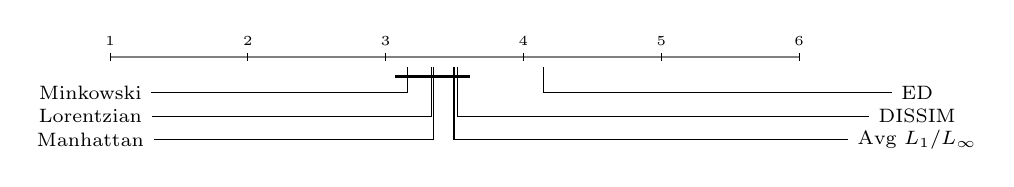
\begin{tikzpicture}[xscale=3]
\draw[gray, thick](00.5833, 0) -- (03.5000, 0);
\foreach \x in {00.5833,01.1667,01.7500,02.3333,02.9167,03.5000}\draw (\x cm,1.5pt) -- (\x cm, -1.5pt);
\node (Label) at (00.5833,0.2) {\tiny{1}};
\node (Label) at (01.1667,0.2) {\tiny{2}};
\node (Label) at (01.7500,0.2) {\tiny{3}};
\node (Label) at (02.3333,0.2) {\tiny{4}};
\node (Label) at (02.9167,0.2) {\tiny{5}};
\node (Label) at (03.5000,0.2) {\tiny{6}};
\draw[decorate,decoration={amplitude=.4mm,segment length=1.5mm,post length=0mm}, very thick, color = black](01.7910,-00.2500) -- ( 02.1051,-00.2500);
\node (Point) at (01.8410, 0){};  \node (Label) at (0.5,-00.4500){\scriptsize{Minkowski}}; \draw (Point) |- (Label);
\node (Point) at (01.9437, 0){};  \node (Label) at (0.5,-00.7500){\scriptsize{Lorentzian}}; \draw (Point) |- (Label);
\node (Point) at (01.9507, 0){};  \node (Label) at (0.5,-01.0500){\scriptsize{Manhattan}}; \draw (Point) |- (Label);
\node (Point) at (02.4197, 0){};  \node (Label) at (4.0,-00.4500){\scriptsize{ED}}; \draw (Point) |- (Label);
\node (Point) at (02.0551, 0){};  \node (Label) at (4.0,-00.7500){\scriptsize{DISSIM}}; \draw (Point) |- (Label);
\node (Point) at (02.0393, 0){};  \node (Label) at (4.0,-01.0500){\scriptsize{Avg $L_{1}$/$L_{\infty}$}}; \draw (Point) |- (Label);
\end{tikzpicture}
\vspace{-0.3cm}
\caption{\textcolor{black}{Ranking of lock-step measures under $z$-score based on the average of their ranks across datasets.}}
\label{john_fig:zscoremanymeasures}
\vspace{-0.5cm}
\end{figure}

\begin{figure} \centering 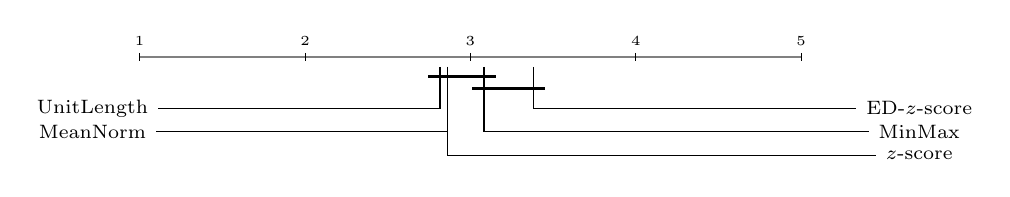
\begin{tikzpicture}[xscale=3]
\draw[gray, thick](00.7000, 0) -- (03.5000, 0);
\foreach \x in {00.7000,01.4000,02.1000,02.8000,03.5000}\draw (\x cm,1.5pt) -- (\x cm, -1.5pt);
\node (Label) at (00.7000,0.2) {\tiny{1}};
\node (Label) at (01.4000,0.2) {\tiny{2}};
\node (Label) at (02.1000,0.2) {\tiny{3}};
\node (Label) at (02.8000,0.2) {\tiny{4}};
\node (Label) at (03.5000,0.2) {\tiny{5}};
\draw[decorate,decoration={amplitude=.4mm,segment length=1.5mm,post length=0mm}, very thick, color = black](01.9212,-00.2500) -- ( 02.2074,-00.2500);
\draw[decorate,decoration={amplitude=.4mm,segment length=1.5mm,post length=0mm}, very thick, color = black](02.1074,-00.4000) -- ( 02.4153,-00.4000);
\node (Point) at (01.9712, 0){};  \node (Label) at (0.5,-00.6500){\scriptsize{UnitLength}}; \draw (Point) |- (Label);
\node (Point) at (02.0013, 0){};  \node (Label) at (0.5,-00.9500){\scriptsize{MeanNorm}}; \draw (Point) |- (Label);
\node (Point) at (02.3653, 0){};  \node (Label) at (4.0,-00.6500){\scriptsize{ED-$z$-score}}; \draw (Point) |- (Label);
\node (Point) at (02.1574, 0){};  \node (Label) at (4.0,-00.9500){\scriptsize{MinMax}}; \draw (Point) |- (Label);
\node (Point) at (02.0041, 0){};  \node (Label) at (4.0,-01.2500){\scriptsize{$z$-score}}; \draw (Point) |- (Label);
\end{tikzpicture}
\vspace{-0.3cm}
\caption{\textcolor{black}{Ranking of normalization methods in combination with the Lorentzian distance based on the average of their ranks across datasets. ED uses $z$-score normalization.}}
\label{john_fig:lorentziandifferentnorms}
\vspace{-0.2cm}
\end{figure}

\noindent \textbf{Debunking $\mathcal{M}1$ and $\mathcal{M}2$: } Our evaluation shows clear evidence that normalization methods other than $z$-score can lead to significant improvements, which debunks $\mathcal{M}1$. Even though for standalone measures, we did not observe significant improvements (e.g.,  ED with MeanNorm vs. ED with $z$-score), that does not reject our hypothesis. We note that the majority of the UCR datasets are in their $z$-normalized form and, therefore, for fairness, we $z$-normalized all datasets, which may have limited this analysis. Despite that, we identified two new distance measures, unknown until now, that only under MinMax and MeanNorm methods outperform ED with $z$-score and, importantly, $z$-score is not suitable for them. Normalizations such as MeanNorm, which combines $z$-score and MinMax methods, seems to perform the best for several measures. Similarly, our analysis shows that distance measures other than ED can lead to significant improvements, which debunks $\mathcal{M}2$. We identified $7$ distance measures that significantly outperform ED. We emphasize that no previous study considered different normalization methods in order to challenge $\mathcal{M}1$, and our findings contradict both previous studies \cite{ding2008querying,giusti2013empirical}, which concluded that there is no significant difference in the accuracy of lock-step measures.

Next, we focus on sliding versions of lock-step measures. 
\vspace*{-0.1cm}
\section{Time-Series Sliding Distances}
\label{john_sec:sliding}

We study $4$ variants of cross-correlation, a measure that has largely been omitted from evaluations. 

Starting with the concurrent introduction of lock-step and elastic measures for the problem of time-series similarity search \cite{agrawal1993,Faloutsos1994fast,berndt1994using}, the vast majority of research focused on these two categories of measures (see $\mathcal{M}3$ in Section \ref{john_sec:perceptions}). Cross-correlation, which is similar to convolution, dates back in the 1700s \cite{dominguez2015history} but received practical popularity only after the invention of Fast Fourier Transform (FFT) \cite{cooley1965algorithm}, which dramatically reduced its computational cost. Cross-correlation is one of the most fundamental operations in signal processing \cite{brown1992survey} and, lately, in deep neural networks \cite{lecun1995convolutional,lecun2015deep}. Recently, research focusing on time-series clustering used cross-correlation and achieved state-of-the-art performance for this task \cite{paparrizos2015k,paparrizos2017fast}. However, this work assumed $z$-normalized time series and performed evaluations only against ED and DTW. (Refer to \cite{paparrizos2015k,paparrizos2020debunking} for the mathematical notation.)
\newline \textbf{Evaluation of sliding measures: } Due to the resemblance of cross-correlation to the sliding version of Pearson's correlation, when time series are $z$-normalized, the majority of the literature assumes this underlying data normalization \cite{paparrizos2015k}. To the best of our knowledge, the performance of cross-correlation as a measure to compare time series under different normalization methods is not well explored. We measure the performance of the combinations of cross-correlation variants with normalization methods. Specifically, from 32 such combinations (i.e., $4$ measures $\times$ $8$ normalizations), we report only those resulted in an average accuracy higher than the one achieved by Lorentzian (with $z$-score followed by UnitLength), the new state-of-the-art lock-step distance measure based on our previous analysis (Section \ref{john_sec:lockstep}). (Refer to \cite{paparrizos2020debunking} for raw numbers and detailed pairwise analysis.)



\begin{figure} \centering 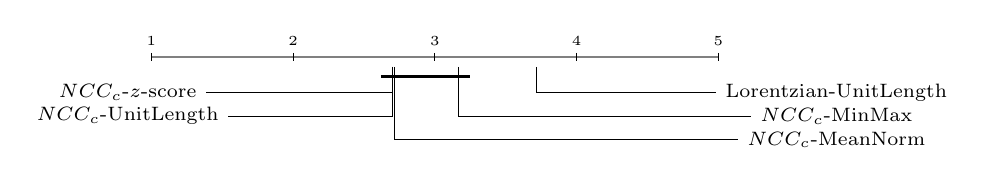
\begin{tikzpicture}[xscale=3]
\draw[gray, thick](00.6000, 0) -- (03.0000, 0);
\foreach \x in {00.6000,01.2000,01.8000,02.4000,03.0000}\draw (\x cm,1.5pt) -- (\x cm, -1.5pt);
\node (Label) at (00.6000,0.2) {\tiny{1}};
\node (Label) at (01.2000,0.2) {\tiny{2}};
\node (Label) at (01.8000,0.2) {\tiny{3}};
\node (Label) at (02.4000,0.2) {\tiny{4}};
\node (Label) at (03.0000,0.2) {\tiny{5}};
\draw[decorate,decoration={amplitude=.4mm,segment length=1.5mm,post length=0mm}, very thick, color = black](01.5718,-00.2500) -- ( 01.9484,-00.2500);
\node (Point) at (01.6218, 0){};  \node (Label) at (0.5,-00.4500){\scriptsize{$NCC_{c}$-$z$-score}}; \draw (Point) |- (Label);
\node (Point) at (01.6218, 0){};  \node (Label) at (0.5,-00.7500){\scriptsize{$NCC_{c}$-UnitLength}}; \draw (Point) |- (Label);
\node (Point) at (02.2290, 0){};  \node (Label) at (3.5,-00.4500){\scriptsize{Lorentzian-UnitLength}}; \draw (Point) |- (Label);
\node (Point) at (01.8984, 0){};  \node (Label) at (3.5,-00.7500){\scriptsize{$NCC_{c}$-MinMax}}; \draw (Point) |- (Label);
\node (Point) at (01.6290, 0){};  \node (Label) at (3.5,-01.0500){\scriptsize{$NCC_{c}$-MeanNorm}}; \draw (Point) |- (Label);
\end{tikzpicture}
\vspace{-0.3cm}
\caption{\textcolor{black}{Ranking of different normalization methods for $NCC_{c}$ based on the average of their ranks across datasets, using Lorentzian with UnitLength as the baseline method.}}
\label{john_fig:sliding1}
\vspace{-0.2cm}
\end{figure}







In addition to these pairwise comparisons, we also evaluate the significance of the differences when considered all together. Figure \ref{john_fig:sliding1} shows the average rank across datasets of five combinations of $NCC_{c}$ with normalization methods. Similarly to the pairwise analysis, we observe that combinations with $z$-score, MeanNorm, and UnitLength normalizations lead to significant improvements according to the Friedman test followed by a post-hoc Nemenyi test to assess the significance of the differences in the ranking. Combinations of $NCC_{c}$ with AdaptiveScaling or MinMax do not achieve significant improvement. We observe that both statistical evaluation approaches lead to similar conclusions.

For completeness, we report another analysis using ED as the baseline instead of the Lorentzian distance (we omit the figure due to space limitation). $NCC_{c}$ in combination with $z$-score, UnitLength, and MeanNorm normalization methods outperform ED but, in contrast to Figure \ref{john_fig:sliding1}, now combinations with AdaptiveScaling and MinMax are also significantly better than ED. This analysis confirms our results in Section \ref{john_sec:lockstep} that the Lorentzian distance (and other $L_{1}$ variants) are more powerful than ED. In addition, our analysis indicates that $NCC_{c}$ outperforms all lock-step measures with all different normalizations, making it a strong baseline method for time-series comparison.

We now turn our focus to elastic measures and their performance against sliding measures.

\section{Time-Series Elastic Measures}
\label{john_sec:elastic}

In this section, we study $7$ elastic measures, a popular category of measures for time-series comparison.

As discussed earlier, sliding measures find a global alignment by sliding one time series against the other. In contrast, elastic measures create a non-linear mapping between time-series data points to support flexible alignment of different regions. Through this mapping, elastic measures permit time series to ``stretch'' or ``shrink'' their observations to improve time-series matching. Most elastic measures rely on dynamic programming to find this mapping efficiently by defining recursive formulas over a $m$-by-$m$ matrix $M$ that contains in each cell the ED (or some other lock-step measure) between every point of one time series against every point of another time series. In general, the goal of different elastic measures in the literature is to employ different strategies to find a {\em warping path}, $W=\{w_1,\ldots,w_k\}$, with $k\geq m$, a contiguous set of matrix cells that shows the mapping of every point of one time series to one, more, or none of the points of the other time series. To improve the efficiency and the accuracy of elastic measures, it is a common practice to introduce constraints (i.e., parameters) to guide the warping path to visit only a subset of cells in $M$.

The first elastic measure, DTW \cite{sakoe1971dynamic,sakoe1978dynamic}, was proposed as a speech recognition tool and, later, it was introduced in the time-series literature as a suitable approach for time-series comparison \cite{berndt1994using}. DTW finds the warping path that minimizes the distances between all data points. In the original form, DTW is parameter-free, however, many approaches have been proposed to define {\em bands} (i.e., the shape of the subset cells of matrix $M$ that the warping path is permitted to visit) and the {\em width or window} (i.e., size) of the bands. We use the Sakoe-Chiba band \cite{sakoe1978dynamic}, which is the most frequently used in practice \cite{ding2008querying}, and we tune the window $\delta$ using parameters shown in Table 4 of \cite{paparrizos2020debunking}. For example, a value $\delta=10$ indicates a window size $10\%$ of the time-series length. 

The Longest Common Subsequence (LCSS) distance is another type of elastic measure that was derived from the idea of edit-distances for characters. Specifically, LCSS introduces a parameter $\epsilon$ that serves as a threshold to determine when two points of time series should match \cite{andre1997using,vlachos2002discovering}. Similarly to DTW, LCSS also constrains the warping window by introducing an additional parameter $\delta$ \cite{vlachos2002discovering}. Edit Distance on Real sequence (EDR) distance \cite{chen2005robust} is another edit-distance-based measure that similarly to LCSS, uses a parameter $\epsilon$ to quantify the distance of points as $0$ or $1$. EDR also introduces penalties for gaps between matched subsequences. Edit Distance with Real Penalty (ERP) distance \cite{chen2004marriage} bridges DTW and EDR distance measures by more carefully computing the distance between gaps.

Differently than the previous approaches, the Sequence Weighted Alignment model (Swale) \cite{morse2007efficient} proposes a model to compute the similarity of time series using rewards for matching points and penalties for gaps. Apart from a threshold $\epsilon$ parameter, Swale also requires parameters for the reward $r$ and the penalty $p$. The Move–split–merge (MSM) distance \cite{stefan2013move} is another elastic measure based on edit-distance but in contrast to DTW, LCSS, and EDR, MSM is a metric. MSM uses a set of operations to replace, insert, or delete values in time series to improve their matching. Finally, Time Warp Edit (TWE) distance \cite{marteau2008time} is a measure that combines merits from LCSS and DTW. TWE introduces a stiffness parameter $\nu$ to control the warping but at the same point it also penalizes matched points.
%For each one of these $7$ elastic measures, several variants and extensions have been proposed in the literature. For example, Derivative DTW (DDTW) \cite{gorecki2013using} combines raw time series with their first-order differences (derivatives). Complexity Invariant distance (CID) \cite{batista2014cid} is a weighting scheme to compensate for differences in the complexity of two time series. Finally, Weighted DTW (WDTW) \cite{jeong2011weighted} adds a penalty to the warping path of DTW. All of these approaches describe extensions that can potentially be used in combination with all previously described elastic measures. Importantly, each of these extensions often introduces additional parameters that require tuning. To avoid an explosion of evaluated approaches, we do not include such variants in our analysis. An excellent recent study \cite{bagnall2017great} focusing on time-series classification has evaluated several of these approaches (and did not identify significant improvements from their use). 
\newline \textbf{Evaluation of elastic vs. sliding measures: } With the introduction of the $7$ elastic measures we are now in position to evaluate their performance against sliding measures, an experiment that has been omitted in all previous studies \cite{ding2008querying,bagnall2017great}. Refer to \cite{paparrizos2020debunking} for detailed raw numbers and pairwise comparisons under supervised and unsupervised settings.

\begin{figure} \centering 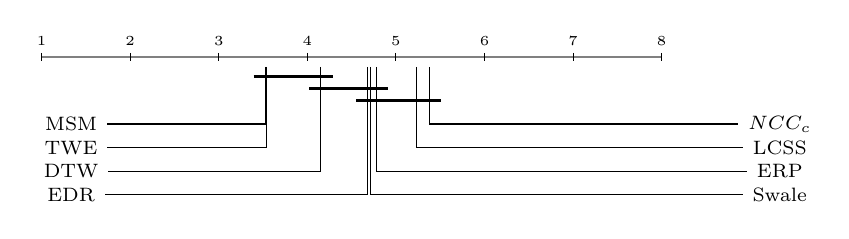
\begin{tikzpicture}[xscale=3]
\draw[gray, thick](00.3750, 0) -- (03.0000, 0);
\foreach \x in {00.3750,00.7500,01.1250,01.5000,01.8750,02.2500,02.6250,03.0000}\draw (\x cm,1.5pt) -- (\x cm, -1.5pt);
\node (Label) at (00.3750,0.2) {\tiny{1}};
\node (Label) at (00.7500,0.2) {\tiny{2}};
\node (Label) at (01.1250,0.2) {\tiny{3}};
\node (Label) at (01.5000,0.2) {\tiny{4}};
\node (Label) at (01.8750,0.2) {\tiny{5}};
\node (Label) at (02.2500,0.2) {\tiny{6}};
\node (Label) at (02.6250,0.2) {\tiny{7}};
\node (Label) at (03.0000,0.2) {\tiny{8}};
\draw[decorate,decoration={amplitude=.4mm,segment length=1.5mm,post length=0mm}, very thick, color = black](01.2726,-00.2500) -- ( 01.6070,-00.2500);
\draw[decorate,decoration={amplitude=.4mm,segment length=1.5mm,post length=0mm}, very thick, color = black](01.5070,-00.4000) -- ( 01.8414,-00.4000);
\draw[decorate,decoration={amplitude=.4mm,segment length=1.5mm,post length=0mm}, very thick, color = black](01.7065,-00.5500) -- ( 02.0656,-00.5500);
\node (Point) at (01.3226, 0){};  \node (Label) at (0.5,-00.8500){\scriptsize{MSM}}; \draw (Point) |- (Label);
\node (Point) at (01.3271, 0){};  \node (Label) at (0.5,-01.1500){\scriptsize{TWE}}; \draw (Point) |- (Label);
\node (Point) at (01.5570, 0){};  \node (Label) at (0.5,-01.4500){\scriptsize{DTW}}; \draw (Point) |- (Label);
\node (Point) at (01.7565, 0){};  \node (Label) at (0.5,-01.7500){\scriptsize{EDR}}; \draw (Point) |- (Label);
\node (Point) at (02.0156, 0){};  \node (Label) at (3.5,-00.8500){\scriptsize{$NCC_c$}}; \draw (Point) |- (Label);
\node (Point) at (01.9627, 0){};  \node (Label) at (3.5,-01.1500){\scriptsize{LCSS}}; \draw (Point) |- (Label);
\node (Point) at (01.7914, 0){};  \node (Label) at (3.5,-01.4500){\scriptsize{ERP}}; \draw (Point) |- (Label);
\node (Point) at (01.7666, 0){};  \node (Label) at (3.5,-01.7500){\scriptsize{Swale}}; \draw (Point) |- (Label);
\end{tikzpicture}
\vspace{-0.3cm}
\caption{\textcolor{black}{Ranking of elastic and sliding distance measures based on the average of their ranks across datasets, using supervised tuning for their parameters.}}
\label{john_fig:elastic1}
\vspace{-0.2cm}
\end{figure}

\begin{figure} \centering 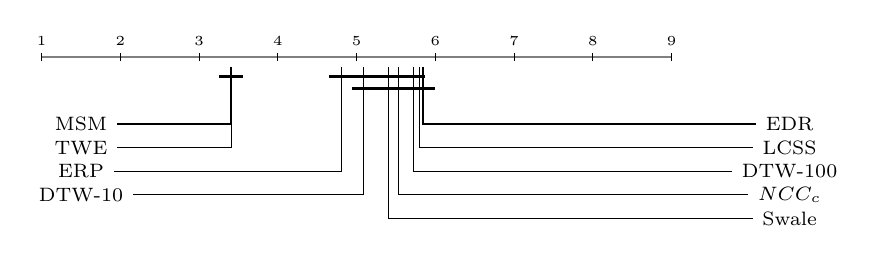
\begin{tikzpicture}[xscale=3]
\draw[gray, thick](00.3333, 0) -- (03.0000, 0);
\foreach \x in {00.3333,00.6667,01.0000,01.3333,01.6667,02.0000,02.3333,02.6667,03.0000}\draw (\x cm,1.5pt) -- (\x cm, -1.5pt);
\node (Label) at (00.3333,0.2) {\tiny{1}};
\node (Label) at (00.6667,0.2) {\tiny{2}};
\node (Label) at (01.0000,0.2) {\tiny{3}};
\node (Label) at (01.3333,0.2) {\tiny{4}};
\node (Label) at (01.6667,0.2) {\tiny{5}};
\node (Label) at (02.0000,0.2) {\tiny{6}};
\node (Label) at (02.3333,0.2) {\tiny{7}};
\node (Label) at (02.6667,0.2) {\tiny{8}};
\node (Label) at (03.0000,0.2) {\tiny{9}};
\draw[decorate,decoration={amplitude=.4mm,segment length=1.5mm,post length=0mm}, very thick, color = black](01.0840,-00.2500) -- ( 01.1853,-00.2500);
\draw[decorate,decoration={amplitude=.4mm,segment length=1.5mm,post length=0mm}, very thick, color = black](01.5517,-00.2500) -- ( 01.9563,-00.2500);
\draw[decorate,decoration={amplitude=.4mm,segment length=1.5mm,post length=0mm}, very thick, color = black](01.6467,-00.4000) -- ( 01.9980,-00.4000);
\node (Point) at (01.1340, 0){};  \node (Label) at (0.5,-00.8500){\scriptsize{MSM}}; \draw (Point) |- (Label);
\node (Point) at (01.1353, 0){};  \node (Label) at (0.5,-01.1500){\scriptsize{TWE}}; \draw (Point) |- (Label);
\node (Point) at (01.6017, 0){};  \node (Label) at (0.5,-01.4500){\scriptsize{ERP}}; \draw (Point) |- (Label);
\node (Point) at (01.6967, 0){};  \node (Label) at (0.5,-01.7500){\scriptsize{DTW-10}}; \draw (Point) |- (Label);
\node (Point) at (01.9480, 0){};  \node (Label) at (3.5,-00.8500){\scriptsize{EDR}}; \draw (Point) |- (Label);
\node (Point) at (01.9323, 0){};  \node (Label) at (3.5,-01.1500){\scriptsize{LCSS}}; \draw (Point) |- (Label);
\node (Point) at (01.9063, 0){};  \node (Label) at (3.5,-01.4500){\scriptsize{DTW-100}}; \draw (Point) |- (Label);
\node (Point) at (01.8437, 0){};  \node (Label) at (3.5,-01.7500){\scriptsize{$NCC_c$}}; \draw (Point) |- (Label);
\node (Point) at (01.8020, 0){};  \node (Label) at (3.5,-02.0500){\scriptsize{Swale}}; \draw (Point) |- (Label);
\end{tikzpicture}
\vspace{-0.3cm}
\caption{\textcolor{black}{Ranking of elastic and sliding distance measures based on the average of their ranks across datasets, using unsupervised tuning for their parameters.}}
\label{john_fig:elastic2}
\vspace{-0.2cm}
\end{figure}


%\textcolor{black}{From Table \ref{john_table:elastic1}, we observe that when parameters are selected under supervised settings (lines with LOOCCV tuning) all elastic measures significantly outperform $NCC_c$ with one exception, the LCSS measure, which marginally outperforms $NCC_c$  but the difference is not statistically significant according to Wilcoxon.} However, the picture is different for the unsupervised scenario. Specifically, we observe that $4$ out of the $7$ elastic measures do not outperform $NCC_c$. Interestingly, LCSS, EDR, and DTW (with $\delta=100$, which resembles an equivalent parameter-free measure to $NCC_c$) are slightly worse. MSM, TWE, and ERP on the other side significantly outperform $NCC_c$ in the unsupervised setting as well. Among all elastic measures, ERP is the only parameter-free measure that achieves significantly better accuracy than $NCC_c$ in both supervised and unsupervised settings.

To understand the performance of elastic measures against $NCC_c$, we evaluate the significance of the differences when considered all together. Specifically, Figure \ref{john_fig:elastic1} shows the average ranks of the elastic measures in the supervised setting and Figure \ref{john_fig:elastic2} shows the average ranks in the unsupervised setting. We observe that even under supervised settings, $4$ out of the $7$ elastic measures, namely, LCSS, ERP, EDR, and Swale, do not achieve significantly better performance than $NCC_c$. The results for MSM, TWE, and DTW, are consistent in both statistical evaluations. For the unsupervised setting, both statistical evaluation approaches agree to an extent. In particular, Figure \ref{john_fig:elastic2} shows clearly that MSM and TWE outperform $NCC_c$. However, the remaining $5$ elastic measures perform similarity to $NCC_c$. \textcolor{black}{To validate our findings, we repeat the analysis (we omit figures due to space limitation) and evaluate the significance of the differences when we consider all elastic measures together (i.e., excluding $NCC_c$). Specifically, we observe that Swale, ERP, EDR, and LCSS do not outperform DTW-10 with statistically significant difference. Interestingly, the supervised LCSS is slightly worse than the unsupervised DTW-10. ERP, which under pairwise evaluation appears to significantly outperform DTW-10, when all measures are considered together, both appear to achieve comparable performance. MSM, TWE, and DTW also perform similarly and all three supervised measures outperform DTW-10. However, under unsupervised settings, MSM and TWE significantly outperform all elastic measures.}

\noindent \textbf{Debunking $\mathcal{M}3$ and $\mathcal{M}4$: } Our comprehensive evaluation shows clear evidence that sliding measures are strong baselines that most elastic measures do not manage to outperform either in supervised or unsupervised settings, which debunks $\mathcal{M}3$. Specifically, from all $5$ elastic measures evaluated in the decade-old study \cite{ding2008querying}, namely, LCSS, Swale, EDR, ERP, and DTW, only DTW significantly outperforms cross-correlation under the supervised scenario. In the unsupervised setting, none of the $5$ measures outperforms cross-correlation and, interestingly, several of them perform slightly worse. This is a remarkable finding, showing that the simplest type of alignment between time series is very effective and it should have served as a baseline method for elastic measures. Only MSM and TWE, two measures that appeared after \cite{ding2008querying} show promising results and outperform cross-correlation with statistically significant differences in both supervised and unsupervised settings. Importantly, MSM is the only method that significantly outperforms DTW under supervised settings (according to Wilcoxon) and, under unsupervised settings, both MSM and TWE significantly outperform DTW (with both statistical tests validating this result). Therefore, there is clear evidence that the widely popular DTW is no longer the best elastic distance measure, which debunks $\mathcal{M}4$. 

%\newline \textbf{Evaluation of elastic measures: } Even though the previous analysis shows some trends about the performance among elastic measures, we repeat the analysis using DTW with $\delta=10$ (DTW-10), a strong elastic measure, for baseline (we omit tables and figures due to space limitation). 

%Table \ref{john_table:elastic2} compares the classification accuracy of elastic measures against DTW with $\delta=10$ (DTW-10). We observe $3$ elastic measures that outperform DTW-10 when parameters are selected under supervision. Specifically, MSM, TWE, and DTW (with LOOCCV tuning) outperform DTW-10 with statistically significant difference. However, LCSS, Swale, and EDR, three supervised elastic measures, achieve comparable performance to DTW-10, an unsupervised measure. As expected, the unsupervised versions of LCSS, Swale, and EDR also do not outperform DTW-10. Interestingly, EDR appears statistically significantly worse than DTW-10 (denoted with \textcolor{NavyBlue}{\ding{74}}). This contradicts the findings of the previous study \cite{ding2008querying}, which concluded that EDR might be potentially slightly better. The unsupervised measures ERP, MSM, and TWE all appear to significantly outperform DTW-10. The DTW-100 version achieves worse performance in terms of average accuracy and, therefore, we do not include it in Table \ref{john_table:elastic2}. However, Wilcoxon suggests that there is no statistically significant differences between the accuracy of DTW-10 and DTW-100.

%To better understand the performance of elastic measures among each other, as before, we also evaluate the significance of the differences when considered all together. Figure \ref{john_fig:elastic3} shows the average ranks among elastic measures in the supervised setting whereas Figure \ref{john_fig:elastic3} shows the average ranks in the unsupervised setting. As before, this analysis contradicts some of the pairwise results in Table \ref{john_table:elastic2}. Specifically, Swale, ERP, EDR, and LCSS do not outperform DTW-10 with statistically significant difference. Interestingly, the supervised LCSS is slightly worse than the unsupervised DTW-10. ERP, which under pairwise evaluation appears to significantly outperform DTW-10, when all measures are considered together, both appear to achieve comparable performance. MSM, TWE, and DTW also perform similarly and all three supervised measures outperform DTW-10. However, the analysis under unsupervised settings show again a different picture (Figure \ref{john_fig:elastic4}). In particular, we observe that MSM and TWE are ranked first, significantly outperforming all other elastic measures.
\vspace{-0.2cm}
\section{Time-Series Kernel Measures}
\label{john_sec:kernel}
\textcolor{black}{Until now, our analysis focused on three categories of distance measures, namely, lock-step, sliding, and elastic measures, with the goal to provide answers to the four-long standing misconceptions that we discussed in Section \ref{john_sec:perceptions}. Recently, kernel functions \cite{scholkopf1997kernel,scholkopf1998nonlinear}, a different category of similarity measures, have started to receive attention due to their competitive performance \cite{abanda2019review}. In contrast to all previously described measures, kernel functions must satisfy the positive semi-definiteness property (p.s.d) \cite{scholkopf2002learning}. The precise definition is out of the scope of this work (we refer the reader to recent papers for a detailed review \cite{abanda2019review,paparrizos2019grail}) but in simple terms, a function is p.s.d. if the similarity matrix, which contains all pairwise similarity values, has positive eigenvalues. This important property results in convex solutions for several learning tasks involving kernels \cite{cortes1995support}. In this section, we study $4$ representative kernel functions and evaluate their performance against sliding and elastic measures.}

\textcolor{black}{Specifically, the first kernel we consider is the Radial Basis Function (RBF) \cite{cristianini2000introduction}, a general purpose kernel function that internally exploits ED but maps data into a high-dimensional space where their separation is easier. To capture similarities between the shifted versions of time series, \cite{wachman2009kernels} proposed a sliding kernel to consider all possible alignments between time-series. We include a recently proposed variant of this kernel, namely, SINK, that has achieved competitive results to $NCC_c$ and DTW \cite{paparrizos2019grail}. Finally, we include two elastic kernel functions, the Global Alignment Kernel (GAK) \cite{cuturi2011fast} and Dynamic Time Warping Kernel (KDTW) \cite{marteau2014recursive}.}

\noindent \textbf{Evaluation of kernel functions: } \textcolor{black}{Having introduced the $4$ kernel functions, we are now in position to evaluate their performance against sliding and elastic measures. As before, we consider both supervised and unsupervised settings. In the supervised setting, we observe that all kernel functions significantly outperform $NCC_{c}$ with the exception of RBF, which is significantly worse. In the unsupervised settings, KDTW and GAK significantly outperform $NCC_{c}$, as before, but SINK achieves comparable performance without outperforming $NCC_{c}$. To better understand the performance of KDTW and GAK, which appear to be the strongest kernel functions, we also evaluate the significance of the differences when considered together with all elastic and sliding measures. Figure \ref{john_fig:kernel2} presents the results for supervised settings and Figure \ref{john_fig:kernel3} for unsupervised settings. We have omitted elastic measures that based on the earlier analysis did not show competitive results. We observe that GAK achieves comparable performance to DTW under both settings. However, KDTW, significantly outperforms DTW in both unsupervised and superivsed settings. This is in contrast to TWE and MSM measures that were significantly better only under the unsupervised settings. To the best of our knowledge, this is the first time that a kernel function is reported to outperform DTW in both settings.}

\begin{figure} \centering 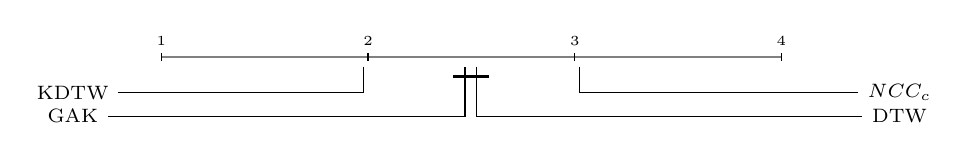
\begin{tikzpicture}[xscale=3]
\draw[gray, thick](00.8750, 0) -- (03.5000, 0);
\foreach \x in {00.8750,01.7500,02.6250,03.5000}\draw (\x cm,1.5pt) -- (\x cm, -1.5pt);
\node (Label) at (00.8750,0.2) {\tiny{1}};
\node (Label) at (01.7500,0.2) {\tiny{2}};
\node (Label) at (02.6250,0.2) {\tiny{3}};
\node (Label) at (03.5000,0.2) {\tiny{4}};
\draw[decorate,decoration={amplitude=.4mm,segment length=1.5mm,post length=0mm}, very thick, color = black](02.1104,-00.2500) -- ( 02.2611,-00.2500);
\node (Point) at (01.7325, 0){};  \node (Label) at (0.5,-00.4500){\scriptsize{KDTW}}; \draw (Point) |- (Label);
\node (Point) at (02.1604, 0){};  \node (Label) at (0.5,-00.7500){\scriptsize{GAK}}; \draw (Point) |- (Label);
\node (Point) at (02.6451, 0){};  \node (Label) at (4.0,-00.4500){\scriptsize{$NCC_c$}}; \draw (Point) |- (Label);
\node (Point) at (02.2111, 0){};  \node (Label) at (4.0,-00.7500){\scriptsize{DTW}}; \draw (Point) |- (Label);
\end{tikzpicture}
\vspace{-0.3cm}
\caption{\textcolor{black}{Ranking of kernel measures based on the average of their ranks across datasets (supervised tuning).}}
\label{john_fig:kernel2}
\vspace{-0.3cm}
\end{figure}


\begin{figure} \centering 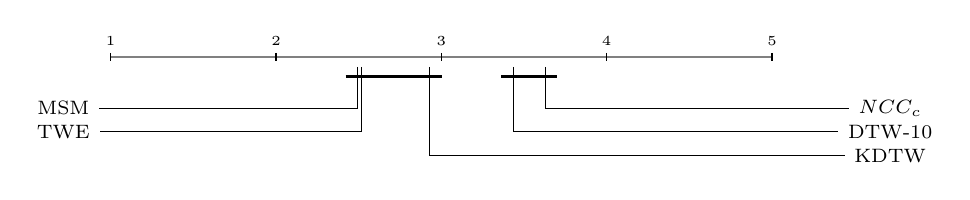
\begin{tikzpicture}[xscale=3]
\draw[gray, thick](00.7000, 0) -- (03.5000, 0);
\foreach \x in {00.7000,01.4000,02.1000,02.8000,03.5000}\draw (\x cm,1.5pt) -- (\x cm, -1.5pt);
\node (Label) at (00.7000,0.2) {\tiny{1}};
\node (Label) at (01.4000,0.2) {\tiny{2}};
\node (Label) at (02.1000,0.2) {\tiny{3}};
\node (Label) at (02.8000,0.2) {\tiny{4}};
\node (Label) at (03.5000,0.2) {\tiny{5}};
\draw[decorate,decoration={amplitude=.4mm,segment length=1.5mm,post length=0mm}, very thick, color = black](01.6944,-00.2500) -- ( 02.1010,-00.2500);
\draw[decorate,decoration={amplitude=.4mm,segment length=1.5mm,post length=0mm}, very thick, color = black](02.3538,-00.2500) -- ( 02.5903,-00.2500);
\node (Point) at (01.7444, 0){};  \node (Label) at (0.5,-00.6500){\scriptsize{MSM}}; \draw (Point) |- (Label);
\node (Point) at (01.7612, 0){};  \node (Label) at (0.5,-00.9500){\scriptsize{TWE}}; \draw (Point) |- (Label);
\node (Point) at (02.5403, 0){};  \node (Label) at (4.0,-00.6500){\scriptsize{$NCC_c$}}; \draw (Point) |- (Label);
\node (Point) at (02.4038, 0){};  \node (Label) at (4.0,-00.9500){\scriptsize{DTW-10}}; \draw (Point) |- (Label);
\node (Point) at (02.0510, 0){};  \node (Label) at (4.0,-01.2500){\scriptsize{KDTW}}; \draw (Point) |- (Label);
\end{tikzpicture}
\vspace{-0.3cm}
\caption{\textcolor{black}{Ranking of kernel measures based on the average of their ranks across datasets (unsupervised tuning).}}
\label{john_fig:kernel3}
\vspace{-0.3cm}
\end{figure}

\section{Time-Series Embedding Measures}
\label{john_sec:embedded}
\textcolor{black}{Previously, we studied approaches that directly exploit a kernel function or a distance measure to compare time series. In this section, we study $4$ embedding measures, which are alternative approaches that employ a similarity measure only to construct new representations \cite{abanda2019review}. These representations are similarity-preserving as the comparison of two representations with ED approximates the comparison of the corresponding original time series with the employed similarity measure.}

\textcolor{black}{We consider $4$ approaches to construct embedding measures (i.e., ED over learned representations). Specifically, we consider the Generic RepresentAtIon Learning (GRAIL) framework, which employs the SINK kernel \cite{paparrizos2019grail}, the Shift-invariant Dictionary Learning (SIDL) method, which preserves alignment between time series \cite{zheng2016efficient}, the Similarity Preserving Representation Learning method (SPIRAL), which employs DTW \cite{lei2017similarity}, and the Random Warping Series (RWS), which preserves the GAK kernel \cite{wu2018random}.}
%\begin{figure} \centering \begin{tikzpicture}[xscale=2]
%\draw[gray, thick](00.7000, 0) -- (03.5000, 0);
%\foreach \x in {00.7000,01.4000,02.1000,02.8000,03.5000}\draw (\x cm,1.5pt) -- (\x cm, -1.5pt);
%\node (Label) at (00.7000,0.2) {\tiny{1}};
%\node (Label) at (01.4000,0.2) {\tiny{2}};
%\node (Label) at (02.1000,0.2) {\tiny{3}};
%\node (Label) at (02.8000,0.2) {\tiny{4}};
%\node (Label) at (03.5000,0.2) {\tiny{5}};
%\draw[decorate,decoration={amplitude=.4mm,segment length=1.5mm,post length=0mm}, very thick, color = black](01.6209,-00.2500) -- ( 01.9092,-00.2500);
%\draw[decorate,decoration={amplitude=.4mm,segment length=1.5mm,post length=0mm}, very thick, color = black](02.6681,-00.2500) -- ( 02.9949,-00.2500);
%\node (Point) at (01.3069, 0){};  \node (Label) at (0.5,-00.6500){\scriptsize{GRAIL}}; \draw (Point) |- (Label);
%\node (Point) at (01.6709, 0){};  \node (Label) at (0.5,-00.9500){\scriptsize{RWS}}; \draw (Point) |- (Label);
%\node (Point) at (02.9449, 0){};  \node (Label) at (4.0,-00.6500){\scriptsize{SIDL}}; \draw (Point) |- (Label);
%\node (Point) at (02.7181, 0){};  \node (Label) at (4.0,-00.9500){\scriptsize{SPIRAL}}; \draw (Point) |- (Label);
%\node (Point) at (01.8592, 0){};  \node (Label) at (4.0,-01.2500){\scriptsize{NCCc}}; \draw (Point) |- (Label);
%\end{tikzpicture}
%\vspace{-0.3cm}
%\caption{\textcolor{black}{Ranking of embedded measures based on the average of their ranks across datasets, using supervised tuning for their parameters.}}
%\label{john_fig:embedded3}
%\vspace{-0.3cm}
%\end{figure}
\newline \noindent \textbf{Evaluation of embedding measures: } \textcolor{black}{For all approaches, we follow \cite{paparrizos2019grail} and tune required parameters using the recommended  values  from  their  corresponding  papers. We construct representations of same length (100) for fairness. We observe that GRAIL, is the only framework that constructs robust representations that when ED is used for comparison (under the 1-NN settings), it achieves similar performance to NCC$_{c}$, but without significant difference. All other embedding measures perform significantly worse and none of the embedding measures outperform DTW (see detailed raw numbers in \cite{paparrizos2020debunking}. We note, however, that embedding measures (as well as kernel methods), achieve much higher accuracy under different evaluation frameworks (e.g., with SVM classifiers), as shown in \cite{paparrizos2019grail}.}

\section{Accuracy-to-runtime Analysis}
\label{john_sec:overall}

Until now, we have extensively evaluated distance measures based on their accuracy results. However, it is also important to understand the cost associated with each one of these distance measures. In Figure \ref{john_fig:accuracyruntime}, we summarize the accuracy-to-runtime performance of the most prominent measures. The runtime performance includes only inference time (i.e., evaluation on the testing sets). We observe that ED, and all other lock-step measures (omitted), are the fastest but achieve relatively low accuracy (all these measures have $\mathcal{O}(m)$ runtime cost). NCC$_c$ \cite{paparrizos2015k} and SINK \cite{paparrizos2019grail}, two methods that rely on the classic cross-correlation measure, provide an excellent trade-off between runtime and accuracy in comparison to ED (these measures have $\mathcal{O}(m \log m)$ runtime cost). We also observe that all other elastic or kernel methods require substantially higher runtime costs to achieve comparable accuracy results to $NCC_c$ (these measures have $\mathcal{O}(m^2)$ runtime cost). In particular, only MSM and TWE significantly outperform $NCC_c$ (see Figure \ref{john_fig:elastic2}) but require two orders of magnitude higher runtime cost. Instead, embedding measures, such as GRAIL \cite{paparrizos2019grail}, show great promise as they can achieve high accuracy without sacrificing runtime performance. %Finally, Figure \ref{john_fig:error} suggests that with increasingly larger dataset sizes the classification error of ED may not always converge to the error of more accurate measures, at least not always with the same speed of convergence, which highlights the importance of considering measures other than ED (see Section \ref{john_sec:perceptions}).


\begin{figure}[t]
	\vspace*{-0.2cm}
	\centering
	\includegraphics[height=8cm,width=15cm]{submissions/John2023/runtime-dis-log.pdf}
	\vspace*{-0.3cm}
	\caption{\textcolor{black}{Accuracy-to-runtime comparison.}}%
	\label{john_fig:accuracyruntime}%
	\vspace*{-0.3cm}
\end{figure}

\section{Accelerating Elastic Measures}
\label{john_sec:accelerating}

Despite their promise, elastic distance measures scale quadratically to the length of the time series, as noted earlier. Compared to ED, which has linear complexity, elastic distance measures incur an additional runtime overhead, often between one to three orders of magnitude (see Figure \ref{john_fig:accuracyruntime}). This cost would prevent applications from using elastic measures in large-scale settings. To alleviate this issue, the idea of {\em lower bounding} was developed to filter out unpromising candidates before carrying out the expensive elastic distance measure computation \cite{kim2001index,keogh2005exact,Faloutsos1994fast}. In simple terms, a lower bound (LB) is a fast distance measure that approximates an expensive elastic distance measure and is computed over some summaries of the time series instead of the actual time series. 

A plethora of LBs have been developed for elastic distance measures \cite{kim2001index,keogh2005exact,shen2018accelerating, tan2020fastee,lemire2009faster,tan2019elastic,chen2004marriage}, with the goal to improve their pruning power (i.e., \textit{tightness} of LB). Unfortunately, the research effort on LBs has been disproportionally concentrated on Dynamic Time Warping (DTW) \cite{sakoe1971dynamic,sakoe1978dynamic}, which is the oldest elastic measure with at least eight established LBs (see \cite{paparrizos2023accelerating} for details). In contrast, newer and better-performing elastic distance measures, such as MSM and TWE, have received little attention, and their LBs are performing poorly. Unfortunately, developing LBs is a challenging task. It is unsustainable to expect a similar research effort for each elastic measure. For this reason, a generalized framework, namely GLB, was recently proposed \cite{paparrizos2023accelerating} to accumulate the knowledge from previously developed LBs and eliminate the need for designing separate LBs for each elastic measure. Specifically, GLB outperforms all established LBs across different elastic measures. Figure \ref{john_fig:pruning} shows the improvement in pruning power (i.e., the percentage of
the true distance computation avoided) achieved by GLB for several popular elastic measures (more details in \cite{paparrizos2023accelerating}). Considering that MSM and TWE are the new state-of-the-art elastic measures, we note that GLB accelerates MSM up to 10$\times$ and TWE up to 26$\times$ in an extensive analysis we performed across 128 datasets \cite{UCRArchive2018}.

\begin{figure}[t]
	\vspace*{-0.2cm}
	\centering
	\includegraphics[height=4cm,width=15cm]{submissions/John2023/figures/selected_pruning.png}
	\vspace*{-0.3cm}
	\caption{\textcolor{black}{Comparison of the pruning power of GLB variants against state-of-the-art LBs of several popular elastic measures over 128 datasets. The blue dots above the diagonal indicate datasets over which GLB outperforms the state of the art.}}%
	\label{john_fig:pruning}%
	\vspace*{-0.3cm}
\end{figure}

%Our extensive experimental evaluation debunked four long-standing perceptions about time-series distance measures that, we believe, significantly alter the landscape of what is known about existing distance measures. In summary, we identified (i) normalization methods that in combination with various ---unknown until now--- distance measures lead to significant improvements in accuracy (e.g., Jaccard with MeanNorm and Emanon4 with MinMax distance measures); (ii) new lock-step measures that significantly outperform ED, the current state-of-the-art lock-step measure (e.g., Lorentzian distance); (iii) an omitted baseline, namely, the cross-correlation measure, that most of the highly popular elastic measures do not outperform; and (iv) new elastic measures, namely, MSM and TWE, that significantly outperform DTW, the current state-of-the-art elastic measure.


%\noindent \textbf{Better than elastic: } Elastic measures currently hold the title of the most accurate distance measures for time-series comparison. However, new categories of distance measures starting being explored (e.g., kernel functions and embedded measures \cite{abanda2019review}). It remains open if any of these types of measures can significantly outperform elastic measures. 

\section{Future Directions}
\label{john_sec:futurework}

With the new knowledge in place, several new challenges open that we hope to spark new research directions. Below, we provide three areas that we believe require more attention and can potentially lead to substantial improvements in the entire area of time-series similarity search:

\begin{itemize}[noitemsep,topsep=0pt,parsep=0pt,partopsep=0pt,leftmargin=0.5cm]
	\item Identifying more accurate normalizations. Our work was the first to study the performance of $8$ normalization methods. We identified multiple distance measures outperforming the previous SOTA measures only when combined with appropriate normalization methods. In our view, inventing a new normalization method that achieves significant accuracy improvements by preprocessing data differently and without changing existing methods and systems would be a breakthrough.
    \item Tuning parameters, or selecting appropriate distance measures per dataset in an unsupervised manner. Unfortunately, there are no principled methodologies currently for selecting distance measures or tuning their parameters, despite significant recent attention in AutoML for other domains.
    \item Improving and evaluating the performance of embedding measures. These measures show the most promise based on their runtime-to-accuracy trade-off. To the best of our knowledge and based on our comprehensive study, there are no embedding measures that significantly outperform the most vigorous elastic measures in terms of accuracy. Recent advances in deep neural networks \cite{wang2023seanet} may lead to embeddings that substantially outperform elastic measures. 
\end{itemize}

\section{Conclusion}
\label{john_sec:conclusions}

We presented a comprehensive evaluation to validate the performance of $71$ distance measures. Our study debunked four long-standing misconceptions in the time-series literature and established new state-of-the-art results for lock-step, sliding, elastic, kernel, and embedding measures. Our findings prepare the ground for the development of distance measures with implications across time-series analytical tasks. Importantly, our work has implications for general-purpose similarity search problems over high-dimensional data. For example, several similarity search methodologies rely heavily on the concepts of lower bounding to prune unnecessary comparisons \cite{paparrizos2022fast,echihabi2018lernaean}. Similarly to how GLB abstracted the costs of different elastic measures and generalized lower bounds for time series, we believe a similar concept can be applied in the case of lock-step measures (e.g., Euclidean distance) and the corresponding data summarization methods. In addition, our work identified lock-step measures that outperform Euclidean distance and lock-step measures performing exceptionally well only under certain normalizations. However, the literature in the similarity search area has largely focused on developing methods assuming Euclidean distance is the underlying distance measure. Our work may lead to new solutions for the new, better-performing distance measures. Finally, the methodologies presented for constructing embedding measures are sufficiently generic and can complement solutions focusing on learning embeddings from data \cite{wang2023seanet} (e.g., concatenate deep embeddings with our similarity-preserving embeddings or improve deep embeddings by integrating our similarity-preserving embeddings in the loss functions).

{\scriptsize  \noindent \textbf{Acknowledgments: }
We thank Kaize Wu for his help and useful discussions. This research was supported in part by a Google  DAPA  Research  Award, gifts from NetApp, Cisco Systems, and Exelon Utilities, and an NSF Award CCF-1139158. Results presented in this paper were obtained using the Chameleon testbed supported by the National Science Foundation.}

%\begin{abstract}
The field of vector search has seen a surge in interest from both researchers and practitioners due to its potential in emerging AI applications. Understanding how to optimize its performance is crucial for numerous tasks, but there remain a lot of challenges in practice. The advent of new hardware architectures and platforms has prompted a reevaluation of the design of large-scale vector search systems. However, current state-of-the-art vector search algorithms have not fully leveraged new hardware architectures to maximize performance.

In this study, we propose design strategies to enhance the computational and memory efficiency of large-scale vector search. Our novel search algorithm, \Hammer, delivers up to an order of magnitude faster search speeds on multi-core architectures through efficient intra-query parallelism, effectively utilizing the combined computational power of modern multi-core chips. Our new design, HM-ANN, employs a novel form of index that effectively leverages heterogeneous memory, enabling billion-scale vector search at a low cost.
This paper delves into the challenges and algorithms associated with \Hammer and HM-ANN, with a focus on improvements in computational and memory efficiency. The paper also includes the results of our experiments that demonstrate the outstanding performance of vector search when modern hardware architectures are effectively utilized through our proposed methods. Lastly, the paper explores open questions and future directions for supporting high-dimensional vector search with speed and scale.

\end{abstract}

%\section{Introduction}\label{sec:intro}

\subsection{Approximate Nearest Neighbor Search}

Finding the top-k nearest neighbors among database vectors for a query has long been a key building block to solve problems such as large-scale information retrieval and image search~\cite{lv2004image, philbin2007object, kulis2009kernelized}, recommendation~\cite{das2007google}, entity resolution~\cite{hoffart2012kore}, and sequence matching~\cite{berlin2015assembling}. As database size and vector dimensionality increase, exact nearest neighbor search becomes expensive and impractical due to latency and memory constraints~\cite{weber1998quantitative, beyer1999nearest, bohm2001searching}. Therefore, to reduce the search cost, various approximate nearest neighbor search (ANNS) algorithms have been proposed to improve efficiency substantially while mildly relaxing accuracy constraints, leading to the so-called accuracy-vs-efficiency tradeoffs. 

Over the years, a variety of algorithms for Approximate Nearest Neighbor Search (ANNS) have been developed with the goal of enhancing computational and memory efficiency. To improve the compute efficiency, well-designed indexes have been introduced, including tree structure-based~\cite{kd-tree,r-star-tree,flann}, hashing-based~\cite{lsh}, and proximity graph-based approaches~\cite{hnsw, nsg}. To improve memory efficiency, various compression algorithms have also been applied to ANNS, such as product quantization-based methods~\cite{product-quantization, opq, cartesian-kmeans, inverted-multi-index, lopq}. These methods can also be combined to improve both compute and memory efficiency simultaneously. For a more detailed understanding and comparison of ANNS algorithms, we recommend several literature that provide excellent surveys~\cite{ann-survey,li2020approximate,wang2021comprehensive}.  

\subsection{Modern Applications and Requirements}

ANNS holds significant relevance in contemporary applications, particularly in conjunction with deep learning models, as it facilitates innovative search scenarios. Traditional entity retrieval relies on keyword matching and user behavior signals. However, with the progression of deep learning, it is now possible to construct models that yield vectors with close distances for entity inputs sharing similar “views”. With these models, one then can encode unstructured data into embedding vectors in a high dimensional space $\mathds{R}^d$~\cite{dssm,multi-field-neural-ranking}. These vectors capture the similarities between various entities within the latent space. As a result, the nearest embeddings for a specific query often symbolize entities with similar semantics in the latent space. ANNS then emerges as a natural choice for managing these vectors while ensuring both speed and accuracy in retrieval.

Vector-based search has already been integrated into many modern applications. For instance, Web-scale search engines like Google~\cite{rankbrain} and Bing~\cite{sptag,diskann} utilize embeddings for documents (e.g., word2vec~\cite{word2vec} and doc2vec~\cite{doc2vec}) and images (e.g., VGG~\cite{vgg}) to retrieve semantically related entities in response to user queries. Major e-commerce players like Amazon~\cite{amazon-search} have developed recommendation systems that embed both the product catalog and the search query, recommending products whose embeddings are closest to the embedded search query. YouTube has built search engine that embeds videos to vectors for video recommendation~\cite{youtube-embed}. More recently, vector search has been employed in retrieval augmented generation in large language models (LLMs), where vector search can be used to expand LLMs knowledge by incorporating external data sources~\cite{retrieval-augmented-generation-deepmind}. Vector search also presents a fertile ground for exploring future applications. For instance, recent advancements in deep learning have enabled models to capture multimodal relationships, such as through the use of multimodal foundation models~\cite{multimodal}. Consequently, the underlying vector search systems can also leverage ANNS to handle multi-modality entities. However, how to effectively handle different modalities and capture the full range of interconnections and relationships among them via ANNS remains an open question. This includes whether various modalities benefit from using the same or different vector search methods, which is an exciting area for future exploration.

As vector search goes to a larger scale, where the dimension scales from $\sim$100 to $\sim$1000 and the number of vectors scales from millions to billions, the challenge of serving latency becomes more prominent even with novel ANNS algorithms. For instance, online interactive services (e.g., web search engine) often require responses to be returned within a few or tens of milliseconds, as delayed responses could degrade user satisfaction and affect revenue~\cite{reduce-web-latency}. However, as the number of entities (such as images and documents) grows rapidly and deep learning embeddings expand to higher dimensions (from embedding sentences to full documents), it becomes increasingly difficult to find highly accurate results in large datasets while adhering to latency constraints. Many vector search services, such as text and image search, require intensive computation and may not be feasible due to latency violations. Therefore, how to transform these applications from impossible to ship due to latency violation to well-fitting SLA is crucial for the practical adoption of vector search. Another big requirement for large-scale vector search is cost reduction. Large-scale services deal with a vast volume of requests and could necessitate thousands of machines for a single application. Therefore, decreasing the number of machines while maintaining the same search quality and latency is crucial for reducing the total cost of ownership for the application.

\subsection{New Hardware Architectures and Opportunities}

Existing ANN algorithms have mostly exploited the uni-core CPU infrastructure and standard memory hierarchy. This infrastructure uses processors whose performance increased with Moore's Law, thus limiting the need for high levels of concurrent execution on a single machine. However, processors are no longer providing ever higher uni-core performance. Meanwhile, the prior infrastructure used DRAM for main memory. However, the main memory capacity is often quite limited to hold a large volume of data. As multi-core processors become ubiquitous and new memory architecture such as heterogeneous memory becomes available, new opportunities for large-scale vector search exist:

\begin{itemize}
    \item \textbf{Design for multi-core}: Modern CPUs are often equipped with high-performance multi-core. Since uni-core speed has pretty much saturated, we need to get better at exploiting a large number of cores by addressing at least two important aspects:
    \begin{enumerate}
        \item Multi-core CPUs provide high concurrency, but as the level of concurrency increases, synchronization among different cores are more likely to block and limit scalability.
        \item The performance of multi-core processes also depend on the shared memory bandwidth utilization. According to the roofline model~\cite{roofline},  the performance of an application is not only bounded by the compute capability but also the bandwidth performance. So how to make the best utilization of memory bandwidth needs great care.
    \end{enumerate} 
    
    \item \textbf{Design for modern memory devices}:  Vector search at large scale is very memory consuming and easily runs out of memory with a few hundred millions of vectors. When the dataset becomes too large to fit on a single machine, one approach is to use the compressed representations of the database points, such as Hamming codes~\cite{hamming-distance} and product quantization~\cite{link-and-code,opq,product-quantization,lopq,cartesian-kmeans}. However, the performance of these methods deteriorates rapidly at higher recall targets, because they calculate approximate distance based on compressed vectors instead of on the original data vectors. Another approach is to exploit storage. In DiskANN~\cite{diskann}, the authors explore slow storage to achieve billion-scale ANNS in a single machine. However, disk latency is a major problem. While persistent media such as SSD offers lower latency and much higher I/O ops per second than traditional disks, they are still several orders of magnitude slower than DRAM. Based on this assumption, data access to the persistent media during search should be minimized. As a result, DiskANN maintains a copy of compressed data in memory with product quantization~\cite{diskann}, which results in loss of in-memory search quality. It then performs a re-ranking using full-precision coordinates stored on SSD, using block-level data accesses but with expensive SSD accessing time. While methods such as DiskANN show promising results, the emergence of Heterogeneous Memory (HM) brings opportunities to significantly improve ANNS. HM combines cheap, slow but extremely large memory with expensive, fast but small memory (e.g., traditional DRAM) to achieve a good balance between production cost, memory performance and capacity. Because of the large memory capacity, HM can use full-precision vectors with accurate distance computation. Since memory access latency/bandwidth of slow memory components in HM is much faster than slow storage such as SSD, it is possible to occasionally access data in slow memory during search without paying the expensive cost of data accesses. That being said, realizing the full performance potential of HM for ANNS is still quite challenging. Although slow memory such as PMM performs $\sim$80X times faster than SSD, it is still $\sim$3X slower than DRAM in terms of random access latency~\cite{pmm-perf}. Therefore, a naive data placement strategy can hurt the search efficiency badly. Therefore, one may still wonder if we can leverage HM for ANNS to achieve both high search accuracy and low search latency, especially when the dataset cannot fit in DRAM (fast memory)?
\end{itemize}

In this work, we revisit the similarity search problem in light of the recent advances in the field. Two new system optimization methods are introduced, dedicated to improving the efficiency and scaling of vector search while simultaneously delivering high accuracy. They are particularly appropriate for the new hardware architectures discussed above. Specially:
\begin{itemize}
    \item iQAN~\cite{iqan} is a parallel search algorithm that exploits intra-query parallelism in graph-based vector search to obtain significant latency reduction in vector search on multi-core architectures with high accuracy. This approach includes a set of optimizations that boost convergence, avoid redundant computations, and mitigate synchronization overhead.
    \item HM-ANN~\cite{hm-ann} is a heterogeneous memory-based technique that shatters the memory barrier of deploying large-scale vector search via NVMe memory, enabling billion-scale vector search with low deployment cost. It carefully constructs vector search indices via a memory hierarchy-aware algorithm, hence leading to substantially better search performance as the vectors grow to be larger than the DRAM capacity. It also employs parallel search algorithms to boost the in-memory search efficiency, leading to faster search speed.    
\end{itemize} 

In drawing broader lessons from this work, we believe that effectively leveraging multi-core and exploiting the memory hierarchy are the keys to high-performance vector search on modern processors. Further, based on the above methods, we discuss open research problems, including exploring hierarchical parallelism to meet both latency and throughput targets, highly concurrent vector search with addition and deletion, automating the index construction for vector search, and the interactions with modern applications in Section~\ref{sec:future}. 







%\vspace{-1em}
\section{Background}\label{minjia_sec:background}

The literature on nearest neighbor search is vast, and hence, we focus our attention on the most relevant works here.  
There has been a lot of work on building effective ANN indices to accelerate the search process. Earlier works focus on space partitioning-based methods. For example, Tree-based methods (e.g., KD-tree~\cite{silpa2008optimised} and R* tree~\cite{r-star-tree}) hierarchically split the data space into lots of regions that correspond to the leaves of a tree structure and only search a limited number of promising regions. However, the complexity of these methods becomes no more efficient than brute-force search as the dimension becomes large (e.g., $>$16)~\cite{worst-case-kdtree}. 
Prior works also have spent extensive efforts on locality-sensitive hashing-based methods~\cite{indyk1998approximate,datar2004locality,andoni2006near,andoni2015practical}, which map data points into multiple buckets with a certain hash function such that the collision probability of nearby points is higher than the probability of others. These methods have solid theoretical foundations. LSH and its variations are often designed for large sparse vectors with hundreds of thousands of dimensions. In practice, LSH-based methods have been outperformed by other methods, such as graph-based approaches, by a large margin on large-scale datasets~\cite{ann-benchmark,hnsw,nsg}. 
More recently, Malkov and Yashunin found graphs that satisfy the small-world property exhibit excellent navigability in finding nearest neighbors. They introduce the Hierarchical Navigable Small World (HNSW)~\cite{hnsw}, which builds a hierarchical k-NN graph with additional long-range links that help create the small-world property. For each query, it then performs a walk, which eventually converges to the nearest neighbor in logarithmic complexity. Subsequently, Fu et al. proposed NSG, which approximates Monotonic Relative Neighbor Graph (MRNG)~\cite{nsg} that also involves long-ranged links for enhancing connectivity. 


% %!TEX root=../2022_IEEE_DEB_Vizier.tex

% %%%%%%%%%%%%%%%%%%%%%%%%%%%%%%%%%%%%%%%%
% \begin{figure}[t]
%   \centering
%   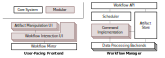
\includegraphics[width=0.7\textwidth]{graphics/systemarch}\\[-5mm]
%   \caption{Vizier's architecture, comprised of a user-facing frontend component and a backend component.}\label{fig:vizier-architecture}
% \end{figure}
% %%%%%%%%%%%%%%%%%%%%%%%%%%%%%%%%%%%%%%%%

%%%%%%%%%%%%%%%%%%%%%%%%%%%%%%%%%%%%%%%%%%%%%%%%%%%%%%%%%%%%%%%%%%%%%%%%%%%%%%%%
\pagebreak[4]
\subsection{Solution Overview}
\label{sec:solution-overview}

%%%%%%%%%%%%%%%%%%%%%%%%%%%%%%%%%%%%%%%%
\begin{wrapfigure}[12]{r}[0pt]{12cm}
  \centering
  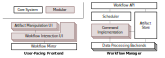
\includegraphics[width=0.7\textwidth]{graphics/systemarch}\\[-5mm]
  \caption{Vizier's architecture, comprised of a user-facing frontend component and a backend component.}\label{fig:vizier-architecture}
\end{wrapfigure}
%%%%%%%%%%%%%%%%%%%%%%%%%%%%%%%%%%%%%%%%
An overview of Vizier's architecture is shown in \Cref{fig:vizier-architecture}.
Addressing requirement \textbf{W1}, the central abstraction in Vizier is a workflow: a linear sequence of steps. % taken by the user in pursuit of a specific objective.
Unlike classical workflow systems, Vizier does not require users to explicitly declare information flow between steps.
Rather Vizier borrows the model employed in popular computational notebooks like Jupyter, where inter-cell communication occurs through a global state (artifacts) passed sequentially through steps.
Following notebook conventions, we refer to these steps as \emph{cells}, and the global state as a \emph{scope}, a map from artifact name to the version of the artifact valid at this point in the workflow. Vizier stores artifacts in common formats through a versioned \textbf{Artifact Store} (\Cref{sec:data-artifacts}), addressing requirement \textbf{A2}.
In \Cref{sec:vizier-workflows}, we formalize Vizier's workflow model, and show how we satisfy requirement \textbf{W3} by instrumenting how each cell interacts with the scope, allowing us to determine what artifact versions are valid.

Vizier's workflow semantics, paired with the versioned artifact store and workflow versioning (\Cref{sec:vizier-history}) addresses requirement \textbf{W2}. % as notebooks have a natural concept of logical order (the order of cells in the notebook) that can be adjusted over time.
% Adding workflow versioning  is sufficient to fully address the requirement.
In contrast, classical notebooks like Jupyter or Zeppelin rely on the global state of an interpreter for inter-cell communication.
Reverting this state to an earlier revision is challenging~\cite{zelnicki:2017:nodebook}, limiting their ability to satisfy requirement \textbf{W3}.
Vizier instead relies on its versioning system, allowing its \textbf{Scheduler} to automatically detect and re-evaluate stale cells (\Cref{sec:vizier-scheduler}).
To address requirement \textbf{A3}, we designed a light-weight uncertain data model that is implemented in Vizier in the form of \textit{caveats}, annotations on data that indicate uncertain values and rows  (\Cref{sec:data-docum-error}).

Addressing requirement \textbf{A1} requires modularity in both Vizier's front- and back-end components.
First, the user's interactions with a workflow and artifacts, whether through a scripting language, graphical interaction, or any other modality, need to be captured for replay (simultaneously addressing requirement \textbf{A4}). In Vizier this is achieved by requiring that every update to an artifact made through a particular modality has to be reflected as an operation in the workflow, i.e., a data update is translated into a workflow update.
Vizier manages a collection of \textbf{Command Implementations} that implement the logic behind these artifact transformations (\Cref{sec:multimodality}).
To streamline the implementation of commands, Vizier's data formats and transformations are built over standard \textbf{Data Processing Backends} like Apache Spark.
% For example, Vizier supports fine-grained provenance over datasets by encoding them as Spark data frames.

The frontend is implemented over a \textbf{Workflow Mirror} that uses websockets to reflect a live view of the workflow the user is editing.
Vizier automatically derives a default \textbf{Artifact Manipulation User Interface} for its notebook interface from each command's parameter schemas. This interface suffices for many templated commands, but the frontend can be further extended to provide a more customized experience, for example for Spreadsheet-style direct manipulation of data (\Cref{sec:spreadsheets}).
As illustrated in \Cref{fig:screenshot}, the frontend displays three \textbf{Workflow Interaction User Interfaces} by default: (i) A direct display of the workflow as a notebook, (ii) a table of contents summary of the notebook, including highlighting from documentation, and (iii) a list of artifacts derived by the notebook.
Several of these components, including the notebook and the artifact list provide access to direct manipulation interfaces.
Additional views currently implemented in Vizier include: (iv) A caveat view (\Cref{sec:data-docum-error}) that shows and tracks potential errors in the workflow and data, (v) a history view that shows the evolution of the workflow over time, and (vi) a data provenance subway diagram view.

%%%%%%%%%%%%%%%%%%%%%%%%%%%%%%%%%%%%%%%%%%%%%%%%%%%%%%%%%%%%%%%%%%%%%%%%%%%%%%%%
\begin{figure}
  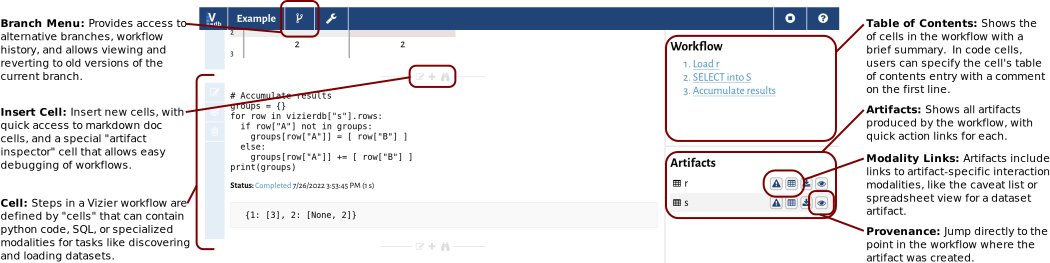
\includegraphics[width=\textwidth]{graphics/screenshot.pdf} 
  \caption{The Vizier User Interface}
  \label{fig:screenshot}
\end{figure}
%%%%%%%%%%%%%%%%%%%%%%%%%%%%%%%%%%%%%%%%%%%%%%%%%%%%%%%%%%%%%%%%%%%%%%%%%%%%%%%%

%%% Local Variables:
%%% mode: latex
%%% TeX-master: "../2022_IEEE_DEB_Vizier"
%%% End:

%\section{iQAN: Fast and Accurate ANNS via Intra-Query Parallelism on Multi-Core Architecture}
\label{sec:iqan}

Among different vector search methods, the similarity graph-based algorithms have emerged as a remarkably effective class of methods for high-dimensional ANNS, outperforming other approaches on a wide range of datasets to achieve the best accuracy-vs-latency~\cite{nsg,ann-benchmark,li2020approximate,echihabi2019return,wei2020analyticdb,wang2020deltapq,product-quantization,babenko2014inverted}. Despite their promising results, graph-based methods still have challenges that limit their use in real-world scenarios.
In particular, as the data size grows, it becomes increasingly challenging to achieve both low latency and high accuracy simultaneously. Existing solutions often resort to inter-query parallelism by dispatching queries across multiple processors or nodes to be processed simultaneously~\cite{nsg,bashyam2020fast}. This approach scales from a throughput perspective, but it does not help reduce query latency because each query still roughly performs the same amount of vector computations to find the nearest neighbors.

\subsection{Challenges of ANNS via Intra-Query Parallelism}

Another natural idea to reduce latency is to exploit intra-query parallelism on individual nodes with multi-core processors. For example, one may parallelize the node expansion in each iteration step of the sequential search algorithm (referred to as \textbf{Node-Expansion-in-Parallel}) because distance computations within a neighborhood expansion iteration do not have dependencies, hoping that multiple worker threads can check the closeness of multiple neighbors in parallel while performing the same computations on each step as the sequential algorithm.  Surprisingly, this solution performs quite poorly and may even perform much worse than a well-tuned sequential algorithm, as shown in Fig.~\ref{fig:insight_edge_wise_latency}. There are several challenges in scaling ANNS with intra-query parallelism:

\textbf{Challenge 1: Modern multi-core hardware is sensitive to synchronization overhead.}
Parallelism boosts compute capacity but may also incur high synchronization overhead, especially if there are complex data dependencies. While parallelizing the distance computation,  Node-Expansion-in-Parallel also requires synchronization in between expansion iterations to sort the distance order of all candidates discovered by multiple parallel workers according to their distances to the query point, to decide which node to expand in the next iteration. We have observed that the synchronization is very expensive on a multi-core architecture, and frequent sequential-to-parallel synchronization as in Node-Expansion-in-Parallel can significantly prolong the search process. 
Fig.~\ref{fig:insight_edge_wise_sync_overhead} shows that as we increase the number of threads, the synchronization overhead accounts for more than 50\%
of the total search time, becoming a dominating factor in the overall search latency. 

\begin{figure}[!ht]
\begin{minipage}[t]{0.23\textwidth}
    \centering
    \includegraphics[height=0.98in]{figures/insight_edge_wise_latency.pdf}
    \caption{
        {EP's latency on Deep100M.}
    }
    \label{fig:insight_edge_wise_latency}
\end{minipage}
\hfill
\begin{minipage}[t]{0.23\textwidth}
    \centering
    \includegraphics[height=0.98in]{figures/insight_edge_wise_sync_overhead}
    \caption{
        {EP adds high sync. overhead.}
    }
    \label{fig:insight_edge_wise_sync_overhead}
\end{minipage}
\hfill
\begin{minipage}[t]{0.23\textwidth}
    \centering
    \includegraphics[height=0.9in]{figures/insight_NSG_convergence_vs_recall}
    \caption{
        {Iteration depths change along with recall.}
    }
    \label{fig:insight_NSG_convergence_vs_recall}
\end{minipage}
\hfill
\begin{minipage}[t]{0.23\textwidth}
    \centering
    \includegraphics[height=0.9in]{figures/insight_NSG_convergence_vs_dataset_sizes}
    \caption{
        {Iteration depths change along with data sizes.}
    }
    \label{fig:insight_NSG_convergence_vs_dataset_sizes}
\end{minipage}
\end{figure}

\textbf{Challenge 2: Node-Expansion-in-Parallel leads to insufficient computation granularity per worker, leading to sub-optimal memory bandwidth utilization.} Node-Expansion-in-Parallel has low compute intensity because (1) unlike matrix multiplication, the point-wise Euclidean distance computation is an operator with low compute intensity, and (2) the number of neighbors to be expanded in one step is limited, given that similarity graphs naturally have low out-degree to avoid the \emph{out-degree explosion problem}~\cite{nsg}. As such, further dividing the distance computation within each neighbor expansion iteration leads to insufficient work for each worker. 

\textbf{Challenge 3: Vector search using graph traversal requires many iterations to converge, resulting in long sequential dependencies between iterations and thus limiting its scalability.}
The number of neighborhood expansion iterations depends on the recall target and the graph size. For example, 
Fig.~\ref{fig:insight_NSG_convergence_vs_recall} shows that as the recall target increases, the number of iterations to find the top-100 nearest neighbors on a hundred million scale dataset {DEEP100M} grows dramatically as the recall target becomes higher (e.g., a $34.6$-time increase from 0.9 to 0.999 recall). 
Fig.~\ref{fig:insight_NSG_convergence_vs_dataset_sizes} shows that as the dataset size increases, the number of iterations to find the results for recall target 0.999 also grows  (e.g., $7.3$ times from 1M-vector dataset to 100M-vector dataset). This long sequential dependency makes achieving low latency with high accuracy especially challenging. 

\subsection{Design of \Hammer}
\label{subsec:iqan-design}

To address the aforementioned challenges, we introduce \Hammer, a parallel search algorithm to accelerate graph-based ANNS on multi-core architectures with three key optimizations: (i) reducing neighbor expansion iteration depth by path-wise parallelism, (ii) reducing redundant distance computation by staged expansion, and (iii) reducing synchronization overhead by redundancy-aware synchronization. 

\subsubsection{Reduce Iteration Depth by Intra-Query Path-Wise Parallelism} 
\label{subsec:path-wise}


In each search iteration, a Best-First-Search (\SeqShortName) algorithm is often used to perform node expansion to the most promising unchecked candidate~\cite{hnsw,nsg}. In \Hammer, we make a small modification to this process by relaxing the priority order and letting each thread expand a few more nodes (e.g., top $W$ unchecked candidates) in every step as active nodes for expansion. We also relax the synchronization such that a global synchronization is only performed after a few expansion steps. We call this new way of expanding nodes \emph{path-wise parallelism (PP)}. This small change in algorithm results in a significant reduction in iteration depths for queries, e.g., from a few {thousands} to {tens} in some cases.

Why would this change reduce the iteration depth? The multi-node expansion and relaxed synchronizations are equivalent to letting each thread explore paths in a local region instead of a single node's neighbor list before doing a global synchronization. By doing so, it increases the likelihood of finding nearest neighbors in less number of iterations. 
Fig.~\ref{fig:insight_convergence_steps_Top_M_vs_SGS} shows the comparison results of iteration depths between \SeqShortName and \emph{PP} on dataset SIFT1M using 10K queries with a $0.90$ recall target. We set $W$ to 64. Overall, while \SeqShortName takes 10.1, 69.4, and 88.1 steps to find the top-1, top-50, and top-100 near neighbor, \emph{PP} only takes 3.4, 5.0, and 5.4 steps on average, respectively, a significant reduction. From the unchecked node's perspective, Fig.~\ref{subfig:insight_unchecked_vs_iters} shows that \emph{PP} also takes much fewer steps to converge to a local optimum (i.e., finish examining all the unchecked vertices) than \SeqShortName. 

\begin{figure}[t]
    \begin{minipage}[t]{0.23\textwidth}
        \centering
        \includegraphics[height=0.9in]{figures/insight_last_update_iter_vs_rank}
        \caption{Iteration depths to find the $K$-th nearest neighbor (x-axis).}
        \label{fig:insight_convergence_steps_Top_M_vs_SGS}
    \end{minipage}
    \hfill
    \begin{minipage}[t]{0.23\textwidth}
        \centering
        \includegraphics[height=0.9in]{figures/insight_unchecked_vs_iters}
        \caption{The number of steps for a search to converge.}
        \label{subfig:insight_unchecked_vs_iters}
    \end{minipage}
        \hfill
    \begin{minipage}[t]{0.23\textwidth}
        \centering
        \includegraphics[height=0.90in]{figures/insight_1T_compt_Top_M_vs_SGS}
        \caption{
            {Aggregated distance computations of \SeqShortName w/ EP and PP, where $W = 64$.}}
        \label{fig:insight_1T_compt_Top_M_vs_SGS}
    \end{minipage}
    \hfill
    \begin{minipage}[t]{0.23\textwidth}
        \centering
        \includegraphics[height=0.90in]{figures/insight_Top_M_compt_steps_vs_M}
        \caption{
            Dist. compt. increases as iter. depths decrease for PP increasing $W$.}
        \label{fig:insight_Top_M_compt_steps_vs_M}
    \end{minipage}
\end{figure}

\subsubsection{Reduce Redundant Computation by Staged Expansion}
\label{subsec:staged-expansion}

Although reducing the iteration depth significantly, does it mean the search process will now get desired speedups on multi-core architectures? The answer is no. The path-wise parallelism reduces iteration depths but at the same time introduces a considerate amount of additional distance computations, especially when the number of parallel workers is large. 
Fig.~\ref{fig:insight_1T_compt_Top_M_vs_SGS} shows that to reach the same recall (0.9--0.999), the path-wise parallelism often needs to perform significantly more distance computations than \SeqShortName (1.3--3.5 times). Moreover, we also observe that although the iteration depths continue to decrease by increasing the concurrent expansion width $W$, the number of distance computations inversely increases, as shown in Fig.~\ref{fig:insight_Top_M_compt_steps_vs_M}. 
The huge amount of redundant computations adversely affects search efficiency as many threads are loading vectors for unnecessary computations, wasting memory bandwidth and compute resources. 

To mitigate it, we investigate the usefulness of path-wise parallelism at different search stages: at which stage does the path-wise parallelism reduce the iteration depths the most? 
We found that overall, in the beginning, since all candidates are far from the query, those early expanded candidates are likely to be discarded by closer ones that are visited later. In other words, candidates expanded and checked at an earlier stage have a high likelihood of becoming unnecessary from a future perspective. As the search moves forward toward the region that has near neighbors, a larger expansion width that covers more search paths can effectively prevent the search from getting stuck at a local minimum.

\begin{figure}[t]
\begin{minipage}[t]{0.23\textwidth}
    \centering
    \includegraphics[height=0.91in]{figures/insight_1T_compt_Scale_M_vs_Top_M_vs_SGS}
    \caption{Dist. computation of \SeqShortName, PP w/o and w/ staged expansion.}
    \label{subfig:insight_1T_compt_Scale_M_vs_Top_M_vs_SGS}
\end{minipage}
\hfill
\begin{minipage}[t]{0.23\textwidth}
    \centering
    \includegraphics[height=0.91in]{figures/insight_unchecked_vs_iter_Top_M_Scale_M}
    \caption{Number of unchecked candidates after each search step. }
    \label{subfig:insight_unchecked_vs_iter_Top_M_Scale_M}
\end{minipage}
\hfill
    \begin{minipage}[t]{0.23\textwidth}
        \centering
        \includegraphics[height=0.97in]{figures/insight_PSS_sync_interval_vs_overhead}
        \caption{
            {Sync. overhead and distance compt. as the sync. interval increases.}}
        \label{fig:insight_PSS_sync_interval_vs_overhead}
    \end{minipage}
    \hfill
    \begin{minipage}[t]{0.23\textwidth}
        \centering
        \includegraphics[height=0.97in]{figures/insight_PSS_update_position_example}
        \caption{A query's average update positions during searching.
        }
        \label{fig:insight_PSS_update_position_example}
    \end{minipage}
\end{figure}

Based on these observations, we propose a \emph{staged expansion (SE)} scheme by gradually increasing the expansion width $W$ and the number of workers every $t$ steps during the search procedure. In practice, we set the starting value of $W$ to 1 and the maximum value as the number of available hardware threads. Then for every $t$ steps (e.g., $t=1$) we double the value of $W$ until $W$ reaches its maximum. Fig.~\ref{subfig:insight_1T_compt_Scale_M_vs_Top_M_vs_SGS} shows the comparison results of path-wise parallelism without and with staged expansion. The staged expansion reduces the number of redundant distance computations significantly, leading to distance computations comparable to \SeqShortName. On the other hand, staged expansion is able to preserve the benefits of path-wise parallelism in terms of obtaining reduced iteration depths, as shown in Fig.~\ref{subfig:insight_unchecked_vs_iter_Top_M_Scale_M}. These results indicate that by performing path-wise parallelism at where they are most effective (i.e., the later phase of the search), the parallel search process can effectively converge with reduced iteration depths and minimal addition of redundant computations among multiple workers.

\subsubsection{Reduce Synchronization Overhead by Redundancy-Aware Synchronization}

The remaining performance challenge in parallel search resides in the synchronization, as we still need to decide when to do synchronization. However, reducing the synchronization overhead for graph-based ANNS is non-trivial.
Fig.~\ref{fig:insight_PSS_sync_interval_vs_overhead} shows that as we skip synchronizations in between search iterations (i.e., increasing the interval between two synchronizations), the synchronization overhead (shown as the ratio to the total time) decreases significantly. However, decreasing synchronization increases distance computations, especially when the synchronization intervals become large. This is because as we increase the synchronization interval, it increases the likelihood that individual workers would search their local but unpromising areas without switching to newly identified promising regions found by other workers. As such, one cannot infinitely delay synchronization, and a small set but useful synchronizations are desired to achieve overall high search efficiency without incurring too many redundant computations.  

Finding such intervals turns out to be non-trivial since the relative distance of a query to its near neighbors changes all the time at different stages. It is also hard to find one fixed synchronization interval for all queries. 
To mitigate the synchronization overhead, \Hammer performs \emph{redundancy-aware synchronization (RAS)}, which allows workers to perform a search with low redundant computations by adding a minimal set of global synchronizations. 
We introduce a metric --- \emph{update positions} --- to capture the redundancy during expansion.
When a worker thread expands an unchecked candidate, its unchecked neighbors are then inserted into the worker's local queue, and we define the update position as the \emph{lowest (best)} position of all newly inserted candidates. Thus, \emph{the average update position} (AUP) is the mean of all update positions of workers. 
Fig.~\ref{fig:insight_PSS_update_position_example} demonstrates how an example query's AUP changes during the search process without doing any global synchronizations. We observe that the AUP increases gradually to be equal to the local queue capacity and remains flat to the end. 
When the AUP is close to the queue capacity, it indicates that a majority of workers are searching areas that cannot find promising candidates to update their local results. Therefore, a high AUP indicates that most workers are doing redundant computations, and it would benefit from a global synchronization such that all workers can focus on searching for more promising areas that have a higher probability of including closer near neighbors. 

%\subsection{Evaluation of \Hammer}
\label{minjia_subsec:iqan-eval}

\Hammer offers significant speedups than two state-of-the-art graph-based ANNS, NSG~\cite{NSGGithub,nsg} and HNSW~\cite{HNSWGithub,hnsw} over several public datasets, including SIFT1M (128D), GIST1M (960D), DEEP10M (96D), DEEP100M (96D), and SIFT100M (128D). We measure the latency and \emph{Recall@100} (R@100), which measures the accuracy of finding the top-100 nearest neighbors for every query.
We conduct our experiments on a workstation with Xeon Gold 6138 (2.00 GHz) with 20 cores and 128 GB DRAM (\emph{Skylake} for short). 

Fig.~\ref{minjia_fig:eval-latency} compares the latency of HNSW, NSG, and \Hammer on Skylake. NSG and HNSW use their sequential search algorithm, whereas \Hammer uses 16 threads on Skylake. Across all five datasets, \emph{\Hammer consistently provides latency speedups over existing sequential-based approaches NSG and HNSW over a wide range of recall targets. }
In particular, the speedups from \Hammer increase as the recall target moves to the high accuracy regime (e.g., from 0.90 to 0.999).
Notably, \Hammer achieves up to $12.9\times$ speedups over NSG on DEEP100M on Skylake, obtaining an incredibly low latency of $<$5ms or $<$3ms at the recall target 0.999 by leveraging aggregated multi-core computation and memory bandwidth resources. This enables vector search with very high accuracy on large-scale graphs, even in extremely interactive online applications. 

\Hammer achieves significant latency speedups mainly for three reasons. First, \Hammer's path-wise parallelism effectively reduces the iteration depths, making the sequential dependencies no longer a major bottleneck. This is particularly critical for a large graph (e.g., DEEP100M) and high recall (e.g., 0.999) as seen in Section~\ref{minjia_subsec:iqan-design} that the iteration depths increase significantly as we either scale the graph size or increase the recall targets. 
Second, the reduced iteration depths do not come at the cost of many redundant computations as \Hammer leverages staged expansion to effectively avoid redundant computations from doing path-wise parallelism. Third, \Hammer significantly reduces the synchronization overhead through redundancy-aware synchronization.
It is also worth mentioning that \Hammer achieves excellent speedups as we increase the dimensionality of the embedding vectors. \Hammer achieves up to $24.9\times$ speedups over HNSW on GIST1M on Skylake. This is higher than the speedups we get on a dataset with a similar scale but much smaller dimensionality (e.g., SIFT1M). \Hammer is able to achieve better speedups on higher dimensional vectors because as the vector dimension increases, the amount of computation workload for the pair-wise distance computation also increases, which allows \Hammer to benefit more from parallel computing. 

\begin{figure*}
    \centering
    \includegraphics[width=0.98\textwidth]{submissions/Minjia2023/figures/eva_runtime_Skylake}
    \caption[Study of Latency]{Latency comparison among HNSW, NSG, and \Hammer on  Skylake (16T).}
    \label{minjia_fig:eval-latency}
    % \vspace{-1em}
\end{figure*}

\textbf{Comparison with DiskANN.} Fig.~\ref{minjia_fig:eva_runtime_recall-1_KNL} compares the latency of DiskANN~\cite{subramanya32diskann} (using 1 thread with its in-memory index) and \Hammer (using 32 threads) for \emph{Recall@1} targets. 
For building its indices of datasets SIFT1M and GIST1M, DiskANN uses $L=125$, $R=70$, $\alpha = 2$, which are the same setting as shown in its paper. For DEEP10M, DiskANN uses $L=100$, $R=100$, $\alpha=1.2$. 
Fig.~\ref{minjia_fig:eva_runtime_recall-1_KNL} shows that \Hammer achieves significant latency speedups over DiskANN, especially for the high recall regime. For example, for recall target 0.999, \Hammer has about $180.5\times$ average speedup on DiskANN among these three datasets.

\begin{figure}[t]
\begin{minipage}[t]{0.55\textwidth}
    \centering
    \includegraphics[width=0.98\textwidth]{submissions/Minjia2023/figures/eva_runtime_recall-1_KNL}
    \caption[Recall@1 Latency]{Recall@1 latency of DiskANN and \Hammer.
    }
    \label{minjia_fig:eva_runtime_recall-1_KNL}
\end{minipage}
\hfill
\begin{minipage}[t]{0.42\textwidth}
    \centering
    \includegraphics[width=0.98\textwidth]{submissions/Minjia2023/figures/eva_sift1b_deep1b_latency}
    \caption[Latency for 1B datasets]{Performance comparison of \Hammer and NSG on two billion-scale datasets SIFT1B (\texttt{bigann}) and DEEP1B. 
        }
    \label{minjia_fig:eva_sift1b_deep1b_latency}
\end{minipage}
\end{figure}


\textbf{Scaling to billion points.}
This experiment is conducted on a machine with a 1.5 TB memory.
It is worth mentioning that even 1.5 TB of memory is not enough to build a 100-NN graph with one billion data vectors. Therefore, we limit the out-degree of NSG
when generating the corresponding NSG index so that the index construction can finish in a reasonable amount of time (e.g.,<10 days). We also note that this is the first time to evaluate an NSG graph at a billion scale as the maximum graph prior work such as NSG evaluated contained less than 100M data points. Fig.~\ref{minjia_fig:eva_sift1b_deep1b_latency} compares the latency of \Hammer and NSG. \Hammer uses up to 64 threads, and the recall target is 0.9. 
When using 64 threads, \Hammer follows the trend of scalability we observed as we increase the graph size and outperform NSG with $11.5\times$ and $16.0\times$ speedup for SIFT1B and DEEP1B, respectively, confirming the excellent scalability of \Hammer on large-scale graphs again. 







%\section{HM-ANN: Efficient Billion-Point Vector Search via Heterogeneous Memory}
\label{minjia_sec:hmann}

This section describes a large-scale vector search solution built on top of Heterogeneous Memory. The HNSW index is modified to make it HM-aware, and the search algorithm is also modified to make the search more efficient. With these modifications, this solution enables fast and highly accurate billion-scale ANNS on HM.

\subsection{Design of \name}

The design of \algoname generalizes HNSW, whose hierarchical structure naturally fits into HM. Elements in the upper layers consume a small portion of the memory, making them good candidates to be placed in fast memory (small capacity); The bottom-most layer has all the elements and has the largest memory consumption, which makes it suitable to be placed in slow memory. Unlike HNSW, where the majority of search happens in the bottom-most layer, elements in the upper layers now have faster access speed, so it is a reasonable strategy to increase the access frequency of the upper layers. On the other hand, since accessing L0 is slower, it is preferable to have only a small portion of it to be accessed by each query. The key idea of \algoname is, therefore, to build high-quality upper layers and make most memory accesses happen in fast memory, in order to provide better navigation for search at L0 and reduce memory accesses in slow memory.

\textbf{Notations.} In the rest of the paper, we let $V$ denote the dataset with $N=|V|$ to build the graph; we refer the graph in the layer $i \in \{0, 1,...,l\}$ of \name as $G_i = (V_i, E_i)$ where $V_i$ is the vertex set and $E_i$ is the edge set. We refer $N_i$ as the number of elements in the layer $i$, and we have $N_i=|V_i|$. Because L0 contains all the elements in the database, we have $V_0 = V$ and $N_0 = N$. Based on the hierarchical structure of \name, we have $ V_i \subsetneq V_{i-1}$.  Similar to the existing effort~\cite{hnsw}, we introduce $M_i$ as the maximum number of established connections for each point $v$ in the layer $i$. For $v \in V$, we let $D(v) $ denote the degree of node $v$, and $D(v) = \sum_{u \in V} m(v,u)$ where $m(v,u)=1$ if there exists a link between node $v$ and node $u$.

\subsubsection{HM-aware Index Construction via Top-Down Insertions and Bottom-up Promotions}

To make the ANNS index aware of HM architecture, we generalize the HNSW construction algorithm to include two phases: a top-down insertion phase and a bottom-up promotion phase.

\textbf{Top-down insertions.}
The top-down insertion phase is the same as HNSW, where we incrementally build a hierarchical graph by iteratively inserting each vector $v$ in $V$ as a node in $G$. Each node will generate up to $M$ (i.e., the neighbor degree) out-going edges. Among those, $M - 1$ are short-range edges, which connect $v$ to its $M - 1$ nearest neighbors according to their pair-wise Euclidean distance to $v$. The rest is a long-range edge that connects $v$ to a randomly picked node, which may connect other isolated clusters. It is theoretically justified that graphs (e.g., L0) constructed by inserting these two types of edges guarantee to have the small world properties~\cite{nsg,small-world-dynamics,hnsw}.

\textbf{Bottom-up promotions.} The goal of the second phase is to build a high-quality projection of L0 elements into the layer $1$ (L1), such that the search in L0 can find the true nearest neighbors of the query with only a few hops. Ideally, \algoname wants to achieve the goal that performing 1-greedy search in L0 is sufficient to achieve high recall, so that the slowdown caused by accessing the slow memory is minimal. A straightforward way to project the L0 elements into L1 is to randomly select a subset of elements in L0 to be L1, similar to what HNSW already does to build upper layers. However, we observe that such an approach leads to poor index quality. As a result, many searches end up happening in L0 (slow memory), causing long search latency. 

\algoname uses a \textit{high-degree promotion strategy}. This strategy promotes elements with the highest degree in L0 into L1. 
From the layer $i$ ($i \ge 2$) to $i+1$, \algoname promotes high-degree nodes to the upper layer with a promotion rate of $1/M$, where $M$ is the maximum number of neighbors for each element (i.e., $M_i = M$, where $i=2...l$). A similar promotion rate setting is used in HNSW~\cite{hnsw} and typical skip list~\cite{skip_list}.
\algoname increases search quality in $L1$ by promoting more nodes from $L0$ to $L1$ and setting the maximum number of neighbors for each element in L1 to $2 \times M$ (i.e., $M_1=2 \times M$).  The number of nodes in upper layers ($N_i$, where $i=1..l$) is decided by available fast memory space. 

The high-degree promotion strategy is based on the following observation. The hub nodes of the graph at L0 are those nodes with a large number of connections (i.e., high degree). In the small world navigation algorithm, a higher degree node provides better navigability~\cite{swg}. Most of the shortest paths between nodes flow through hubs. In other words, the average length of the navigation path (i.e., number of hops) is the smallest, when the adjacent node with the highest degree is selected as the next hop. By promoting the high-degree nodes, the resulting L1 layer allows \algoname to effectively reduce the number of search steps in L0, compared with the random promotion strategy.

\subsubsection{\name Graph Search Algorithm}
\label{minjia_sec:searching}

\textbf{Fast memory search.} The search in fast memory begins at the entry point in the top layer and then performs a 1-greedy search from the top layer to layer 2, which is the same as in HNSW. To narrow down the search space in L0, \name performs the search in L1 with a search budget controlled by $efSearch_{L1}$. $efSearch_{L1}$ defines the size of dynamic candidate list in L1. Those candidates in the list are used as entry points for search in L0 (HNSW uses just one entry point), in order to improve search quality in L0. 

\textbf{Parallel L0 search.} In L0, \name evenly partitions the candidates from searching L1 and uses them as entry points to perform \emph{parallel multi-start 1-greedy search} with  $Thr$ threads in parallel. The top candidates from each search are collected to find the best candidates. Parallel search makes the best use of memory bandwidth and improves search quality without increasing search time. $Thr$ is determined by peak memory bandwidth constrained by hardware divided by memory bandwidth consumption by one thread, which is easy to calculate. 

Different from the SSD-based ANNS~\cite{diskann,grip}, the data in slow memory in \name can be directly accessed by processors, and there is no duplication between fast and slow memories. However, due to high latency and low bandwidth of slow memory, \name should still make memory accesses in fast memory as many as possible. \name implements a software-managed cache in fast memory to prefetch data from slow memory to fast memory before the memory access happens. In particular, \name reserves a space in fast memory ($\sim$2 GB) called \textit{migration space}. When searching L1, \name asynchronously copies neighbor elements of those candidates in $efSearch_{L1}$ and the neighbor elements' connections in L1 from slow memory to the migration space in fast memory. When the search in L0 happens, there is already a portion of to-be-accessed data placed in fast memory, which leads to shorter query time.

%\subsection{Evaluation of \name}
\label{subsec:eval-hmann}

\textbf{Billion-scale algorithm comparison.} We compare \algoname with the graph- (HNSW and NSG) and quantization-based algorithms (IMI+OPQ and L\&C).
For HNSW, we build graphs with $efConstruction$ and $M$ set to 200 and 48 respectively; For NSG we first build a 100-NN graph using Faiss~\cite{faiss} and then build NSG graphs with R = 128, L = 70 and C = 500. 
We collect results on NSG and HNSW using Memory Mode since it leads to overall better performance than using first-touch NUMA.
For IMI+OPQ, we build indexes with 64- and 80-byte code books on BIGANN and DEEP1B respectively. We present the best search result with search parameters nprobe=128 and ht=30 for BIGANN and with autotuning parameter sweep on DEEP1B. For L\&C,  we use 6 as the number of links on the base level, and use 36- and 144-byte OPQ code-books. We use the same parameters ($efConstruction$=200 and $M$=48) as HNSW to construct \name. We set $efSearch_{L0}$=2 and vary $efSearch_{L1}$ to show the latency-vs-recall trade-offs.

Figures~\ref{fig:billion} (a)-(d) visualize the results. Overall, \algoname provides the best latency-vs-recall performance. Figure~\ref{fig:billion} (a) and (b) show that \algoname achieves the top-1 recall of $>95\%$ within 1ms, which is 2x and 5.8x faster than HNSW and NSG to achieve the same recall target respectively.  
IMI+OPQ and L\&C cannot reach a similar recall target, because of precision loss from quantization. As another point of reference, the SSD-based solution, DiskANN~\cite{diskann} (not open-sourced), provides 95\% top-1 recall in 3.5ms. In contrast, \name provides the same recall in less than 1ms, which is at least 3.5\(\times\) faster.
We compare the top-100 recall shown in Figures~\ref{fig:billion} (c) and (d). \algoname provides higher performance than all other approaches. For example, it obtains top-100 recall of $>90\%$ within 4 ms, while performing 2.8x and 5x faster than HNSW and NSG with the same recall target respectively. Quantization-based algorithms perform poorly and have difficulties to reach a top-100 recall of 30\%. 

\begin{table}
\newcommand{\colspc}{\hspace*{0.4em}}
\caption{Indexing time and memory consumption for graph-based methods on billion-scale datasets}\label{tab:indexing_time_and_mem_for_1b}
\centering
\scriptsize
\begin{tabular}{|@{\colspc}c@{\colspc}|@{\colspc}c@{\colspc}|@{\colspc}c@{\colspc}|@{\colspc}c@{\colspc}|@{\colspc}c@{\colspc}|@{\colspc}c@{\colspc}|@{\colspc}c@{\colspc}|@{\colspc}c@{\colspc}|@{\colspc}c@{\colspc}|@{\colspc}c@{\colspc}|@{\colspc}c@{\colspc}|}
\hline
\multirow{3}{*}{}                   & \multicolumn{5}{c|}{\textbf{BigANN}}  & \multicolumn{5}{c|}{\textbf{DEEP1B}}               \\ \cline{2-11} & \multicolumn{3}{c|}{\textbf{Indexing}}      & \multicolumn{2}{c|}{\textbf{Search}}                      & \multicolumn{3}{c|}{\textbf{Indexing}}                    & \multicolumn{2}{c|}{\textbf{Search}}                    \\ \cline{2-11} & \centering \begin{tabular}[c]{@{}c@{}}Graph\\  size\end{tabular} &\centering \begin{tabular}[c]{@{}c@{}}Indexing\\  time\end{tabular} & \begin{tabular}[c]{@{}c@{}}Promo.\\  rate\end{tabular} & \centering \begin{tabular}[c]{@{}c@{}}Fast-mem \\ usage\end{tabular} & \begin{tabular}[c]{@{}c@{}}Slow-mem\\  usage\end{tabular} & \begin{tabular}[c]{@{}c@{}}Graph\\  size\end{tabular} & \begin{tabular}[c]{@{}c@{}}Indexing\\  time\end{tabular} & \begin{tabular}[c]{@{}c@{}}Promo.\\  rate\end{tabular} & \centering \begin{tabular}[c]{@{}c@{}}Fast-mem \\ usage\end{tabular} & \begin{tabular}[c]{@{}c@{}}Slow-mem\\ usage\end{tabular} \\ \hline
\multicolumn{1}{|c|}{\textbf{HNSW}} & 475GB  &\centering 90h    &\centering 0.02    & \begin{tabular}[c]{@{}c@{}}96GB\\  (hw caching)\end{tabular}  &\centering 490GB  &\centering 723GB   & \centering 108h &\centering 0.02  & \begin{tabular}[c]{@{}c@{}}96GB\\  (hw caching)\end{tabular} &\centering 748GB  \tabularnewline \hline
\multicolumn{1}{|c|}{\textbf{NSG}}  & 285GB   &\centering 115h &\centering -   & \begin{tabular}[c]{@{}c@{}}96GB\\  (hw caching)\end{tabular} &\centering 303GB  & 580GB  &\centering 134h &\centering -   & \begin{tabular}[c]{@{}c@{}}96GB\\  (hw caching)\end{tabular}  &\centering 599GB   \tabularnewline \hline
\multicolumn{1}{|c|}{\textbf{\name}} & 536GB    &\centering 96h  &\centering 0.16  & \centering 96GB &\centering 462GB  & 756GB  &\centering 117h  &\centering 0.11 &\centering 96GB   &\centering 681GB               \tabularnewline \hline
\end{tabular}
\end{table}

Table~\ref{tab:indexing_time_and_mem_for_1b} shows the index construction time and index size of HNSW, NSG, and \name. Among the three, HNSW takes the shortest time to build the graph. \name takes 8\% longer time than HNSW because it takes an additional pass for the bottom-up promotion. However, \name is still faster to construct than NSG.
In terms of memory usage, \name indexes are 5--13\% larger than HSNW, because it promotes more nodes from L0 to L1. %(i.e., higher promotion rates).
In terms of memory usage, \name consumes less fast memory than HNSW and NSG, which is valuable to reduce production cost~\cite{ram_price,ram_price2}.
HNSW and NSG use all fast memory because they do not explicitly manage HM and by default using Memory Mode consumes all fast memory. The sum of slow and fast memory consumption can be larger than the index size because there are metadata needed for search that are not counted in the index size.

\begin{figure*}[!ht]
 \centering
 \includegraphics[width=\linewidth]{figures/billion_result.pdf}
 \caption{Query time vs. recall curve in (a) DEEP1B top-1, (b) BigANN top-1, (c) DEEP1B top-100, (b) BigANN top-100, respectively.}\label{fig:billion}
\end{figure*}
% \section{Related Work}
\label{sec:related-work}
\noindent \textbf{Pseudo-relevance feedback:} Our method has similarities with %the existing approach of 
Pseudo-Relevance Feedback (PRF) \cite{rocchio1971relevance, lv2009adaptive, li2022does} in IR: \cite{bendersky2011parameterized, xu2017quary} use the retrieved documents to improve sparse approaches via query expansion or query term reweighting, \cite{li2018nprf, zheng2020bert} score similarity between a target document and a top-ranked feedback document, while \cite{yu2021improving} train a separate query encoder that computes a new query embedding using the retrieved documents as additional input. In contrast, our approach does not require customized training feedback models or availability of explicit feedback data, as we improve the query vector by directly distilling from the reranker's output within an R\&R framework. %\pradeep{Why is our approach better?} 

Further, previous approaches to PRF have been dependent on the choice of retriever architecture and language; \cite{yu2021improving}'s PRF model is tied to the retriever used, \cite{chandradevan2022learning} explore cross-lingual relevance feedback, but require feedback documents in target language and thereby could only apply to three languages, while \cite{li2022interpolate} explore interpolating relevance feedback between dense and sparse approaches.
On the other hand, our approach is independent of the choice of the retriever and reranker architecture, and can be used for neural retrieval in any domain, language or modality. \\

\noindent \textbf{Distillation in Neural IR:} Existing approaches primarily leverage reranker feedback \textit{during training} of the dual-encoder retriever, to sample better negatives \cite{qu2021rocketqa}, for standard knowledge distillation of the cross-attention scores \cite{izacard2020distilling}, to train smaller and more efficient rankers by distilling larger models \cite{hofstatter2020improving}, or to align the geometry of dual-encoder embeddings with that from cross-encoders \cite{wang2021enhancing}. Instead, we leverage distillation at inference time, updating only the query representation to replicate the cross-encoder’s scores for the corresponding test instance.
A key implication of this design choice is that unlike existing methods, we keep the retriever parameters unchanged, meaning \textsc{ReFIT} can be incorporated out-of-the-box into any neural R\&R framework. In contrast, extending training-time distillation to new languages or modalities would require re-training the bi-encoder.

More recently, \textsc{TouR}~\cite{sung2023optimizing} has proposed test-time optimization of query representations with two variants: \textsc{TouR}$_{\text{hard}}$ and  \textsc{TouR}$_{\text{soft}}$. 
\textsc{TouR}$_{\text{hard}}$ optimizes the marginal likelihood of a small set of (pseudo) positive contexts.
\textsc{ReFIT} shares similarities with \textsc{TouR}$_{\text{soft}}$, which uses the normalized scores of a cross-encoder over the retrieved results as soft labels.
Crucially, \textsc{TouR} relies on multiple iterations of relevance feedback via distillation, where each iteration runs until the top-1 retrieval result has the highest reranker score (in \textsc{TouR}$_{\text{soft}}$) or is a pseudo-positive (in \textsc{TouR}$_{\text{hard}}$).
This makes inference highly computationally expensive, as each additional iteration involves labeling top-$K$ retrieval results with a reranker and then retrieving again.
\textsc{ReFIT} improves efficiency over \textsc{TouR} by requiring only a single iteration of feedback that simply updates the query vector for longer, foregoing additional retrieval and reranking steps. More specifics on the inference process of the two methods can be found in \S{\ref{sec:tour_comparison}}.
\textsc{TouR} was evaluated only on English phrase and passage retrieval tasks, while we demonstrate \textsc{ReFIT}'s effectiveness in multidomain, multilingual and multimodal settings, with an empirical comparison with \textsc{TouR} in \S{\ref{sec:tour_comparison}}.
%\section{Research Opportunities}
\label{minjia_sec:future}

In this paper, we have concentrated on the computational and memory efficiency of large-scale vector search. Our \Hammer and HM-ANN designs achieve exceptional performance. However, large-scale vector search still requires further attention, and we expect that additional improvements can be made. This section explores the challenges and research opportunities associated with vector search.

\textbf{High-performance vector search through hierarchical parallelism.} Inference demand varies across different applications and scenarios, with some being latency-critical, and others being latency-sensitive or throughput-oriented. Additionally, the hardware resources available to each application may also vary significantly. To meet these diverse requirements and make efficient use of all computational resources, we can combine different parallelism approaches:
\begin{itemize}
    \item Distributed vector search. Libraries such as Milvus~\cite{milvus} allow the development of distributed versions of vector search systems using a cluster.
    \item Inter-query parallelism. Multithreading enables the use of multiple cores to improve the throughput of answering user requests.
    \item Intra-query parallelism. Methods such as \Hammer enable the system to speed up individual queries by leveraging the aggregated computational capacity of multiple cores.
\end{itemize}

These techniques can be combined hierarchically to meet given latency, throughput, and cost objectives. The research opportunity here is: \emph{Build systems for large-scale vector search that fully exploit parallelism at different levels, providing millisecond-level latency, high throughput, and low hardware cost.}
Furthermore, while techniques such as \Hammer optimize search efficiency by modifying the graph traversal process to leverage intra-query parallelism, the underlying index has not been specifically designed to take advantage of intra-query parallelism. Intuitively, a different index structure could achieve better search efficiency under intra-query parallelism if it naturally helps avoid redundant computations across different threads and also leads to better data locality. The research opportunity here is: \emph{Design vector search indices that maximize search efficiency through both inter- and intra-query parallelism. } 

\textbf{Highly concurrent vector search with addition and deletion.} Most existing vector search systems build indices offline and become read-only once deployed. In some applications, data capture may occur more frequently than query processing, or the application may need to index continuous data streams while serving query requests. In these cases, the index organization should be optimized for addition and update in addition to query performance. The complexity arises with concurrent read and update operations (e.g., addition, deletion), as it is challenging to achieve both correctness and speed simultaneously. Concurrent updates and reads can lead to data races, making it difficult to ensure correctness on shared-memory architectures. Lock-based synchronization can be used to coordinate access to shared-memory data, but while using one lock for the entire index simplifies reasoning about correctness, it also leads to serialized execution, severely impacting scalability. Another solution is to use fine-grained locking, where multiple locks are associated with the index. However, fine-grained locking increases the complexity of operations that access shared data, leading to issues such as deadlock, atomicity violation, and high locking overhead. The research opportunity here is: \emph{Build a highly concurrent vector search system that supports robust addition and deletion with high search efficiency}. 

\textbf{Automating index construction for vector search.} Several advances have been made in support of large-scale vector search, introducing novel algorithms and system optimizations~\cite{grip,diskann,hm-ann,spann}. However, applying these methods to large-scale datasets still requires a significant amount of engineering effort specific to the data, hardware environment, and performance objectives. For instance, deploying a large dataset to a given cloud VM requires a careful selection of vector search indices, with NVMe/SSD/remote storage, the number of cores to use, and multiple index-specific parameters. Correctly choosing the algorithm and tuning the parameters can deliver significant improvements in search performance but also depend on strong system expertise. Therefore, automating the selection and construction of vector search indices would help alleviate the burden on deployment engineers, but it also requires navigating a complex space of choices that grows exponentially with different algorithm choices, each with its own trade-offs, and data sizes and hardware resources. The research opportunity here is: \emph{Build a framework and optimization algorithm that automatically finds the optimal index construction strategy for a given dataset to deliver fast search speed with low cost.}


%\vspace{-1em}
\section{Conclusion}\label{sec:conclusion}

We have designed and implemented \Hammer and \name to enhance the system efficiency of vector search. We have followed the state-of-the-art vector search algorithm, but at every level, we have introduced innovations that stretch prior methods and tailor our system for the newer hardware setting of multi-core processors and heterogeneous memory. 
Our innovations, such as intra-query path-wise parallelism, staged expansion, redundancy-aware synchronization, and HM-aware index construction, improve the computational and memory efficiency of large-scale vector search. Many of these methods should work well in other settings, such as SSD-based methods and compression-based indices. Finally, we propose several open research directions from a system perspective that have the potential to further improve large-scale vector search. We hope these directions will inspire new research that can advance vector search and make it more efficient, robust, and easy-to-use.
%\section{Conclusion}\label{sec:conclusions}
Alternative job arrangements such as online job platforms are becoming increasingly important
and a major source of employment in the near future.
It is important for the crowdsourcing community to take the lead on researching the Feature of Work.
In this article, we argue that a key pre-requisite is the creation of benchmarks for such research.
The diversity of crowdsourcing research by various communities is a key challenge.
We propose a taxonomy of dimensions for which benchmarks has to be developed.
We also have enumerated a list of metrics that are most relevant for effective crowdsourcing. Moreover, we list essential factors that need to be considered during the process of creating benchmarking data to test the effectiveness and robutness of crowdsouring platforms. Benchmarks have had a dramatic impact in the development of various domains.
We issue a call-to-arms to the crowdsourcing community to seize the opportunity!


% \begin{thebibliography}{10}
% \itemsep=1pt
% \begin{small}

% \bibliography{bib/ref.bib,bib/refnew.bib}

% \end{small}
% \end{thebibliography}

%\small
\footnotesize 
\bibliographystyle{plainnat} % We choose the "plain" reference style
\bibliography{submissions/John2023/sample-bibliography} % Entries are in the refs.bib 

\end{document}